\documentclass[a4paper,12pt]{article}
\usepackage{fancyhdr}
\usepackage{t1enc}
\usepackage[utf8]{inputenc}
\usepackage[magyar]{babel}
\usepackage{lmodern}
\usepackage[pdftex]{graphicx}
\usepackage[lflt]{floatflt}
\usepackage{epstopdf}
\usepackage{amsmath,amssymb}
\usepackage{icomma}
\usepackage{array}
\usepackage[unicode,colorlinks]{hyperref}
\usepackage{fullpage}
\usepackage{booktabs}
\usepackage{graphicx}
\usepackage[justification=centering]{caption}
\usepackage{subcaption}

\hypersetup{allcolors=black}
\hypersetup{pdfstartview=FitH}
\hypersetup{pdfinfo={
	Title={},
	Author={},
	Subject={},
	Keywords={}
}}

\title{\bf Hanghullámok spektrumanalízise myDAQ mérőkártyával}
\author{ {Bertesina Zeno}, {Bodoky Lukács}, {Hajdú Csanád} }
\date{2020.\ 01.\ 31.}

\topmargin = 0pt
\headheight = 14.5pt
\headsep = 14.5pt

\pagestyle{fancy}
\lhead{\small {\bf Hanghullámok spektrumanalízise myDAQ mérőkártyával}}
\rhead{2020.\ 01.\ 31.}


\widowpenalty=10000 \clubpenalty=10000


% a '\D'-t lehet használni deriválásnál, vagy integrálásnál d-nek
\newcommand{\D}{\mathrm{d}}
% a '\V{...}'-val lehet vektormennyiséget csinálni
\newcommand{\V}[1]{\mathbf{#1}}
% kg/m^3
\newcommand{\kgm}{\frac{\mathrm{kg}}{\mathrm{m}^3}}

\DeclareMathOperator{\tg}{tg}


% ================================================================
\begin{document}

\maketitle
\thispagestyle{empty}

\renewcommand{\abstractname}{Absztrakt}
\begin{abstract}
\noindent A kísérletek célja a magyar nyelvben lévő magánhangzók frekvenciaspektrumának vizsgálata Fourier transzformáció segítségével és különböző húrok vastagságának meghatározása a hangjának alapfrekvenciájából.
\end{abstract}

% ================================================================
\section{Elméleti bevezető}

A később elvégzendő kísérletek a hanghullámok és ezeknek Fourier spektrumának vizsgálatával kapcsolatosak, így ezek elméleti hátterét röviden tárgyaljuk itt.

% ----------------------------------------------------------------
\subsection{Hullámok}

A kiterjedt rugalmas testekben a tapasztalat szerint zavar tud terjedni. Ezt a zavart hullámnak nevezzük. Általánosan egy ilyen zavar terjedését nagyon nehéz, vagy lehetetlen leírni, viszont bizonyos feltevésekkel jelentősen egyszerűsödhet a probléma. Ha feltesszük, hogy az egyes tömegpontok kitérése elég kicsi ahhoz, hogy a visszatérítő erő lineáris legyen, levezethető egy hullámegyenlet,
\begin{equation}
\Delta \Psi(\V{r}, t) = \frac{1}{c^2} \frac{\partial^2 \Psi(\V{r}, t)}{\partial t^2},
\label{hullamegyenlet-3D}
\end{equation}
ahol $\Psi(\V{r}, t)$ a hullámfüggvény, $\Delta$ a Laplace operátor és $c$ a hullám terjedési sebessége. Egy dimenziós esetben az egyenlet
\begin{equation}
\frac{\partial^2 \Psi(x, t)}{\partial x^2} = \frac{1}{c^2} \frac{\partial^2 \Psi(x, t)}{\partial t^2}
\label{hullamegyenlet-1D}
\end{equation}
alakú. $c$ bizonyos esetekben elméleti megfontolásokkal levezethető. A hullámfüggvény egyik egyszerű megoldása a síkhullám,
$$ \Psi (\V{r}, t) = A \cdot \sin (\omega t - \V{k} \V{r} + \varphi) \quad \text{és} \quad \Psi(x, t) = A \cdot \sin(\omega t - k x + \varphi). $$
A függvényben szereplő mennyiségek:
\begin{itemize}
\item $A$ a hullám amplitúdója, a rezgés során a legnagyobb kitérés ([$A$] = m);
\item $\omega$ a körfrekvencia, $\omega = 2 \pi f$, ahol $f$ a rezgés frekvenciája ([$\omega$] = s$^{-1}$, [$f$] = Hz);
\item $\V{k}$ a hullámszám vektor, a hullám terjedési irányába mutat és a $\lambda$ hullámhosszal fordítottan arányos ([$\V{k}$] = m$^{-1}$);
\item $\V{r}$ a közeg adott pontjának helyvektora ([$\V{r}$] = m);
\item $\varphi$ a rezgés kezdőfázisa ([$\varphi$] = $1$);
\end{itemize}

A fentieken kívül más mennyiségeket is tudunk definiálni. A hullámhossz a hullám két azonos fázisú pontja közti távolság, amit $\lambda$-val jelölünk, és ez adja meg a hullám térbeli periodicitását. A közegben egy adott tömegpont is periodikusan mozog, amit a $T$ periódusidővel tudunk jellemezni. Ezzel a hullám terjedési sebessége kifejezhető,
$$ c=\frac{\lambda}{T}. $$
Ennek oka az, hogy két azonos fázisú pont $n T$ idővel van eltolva egymástól és pontosan $n \lambda$ távolságra vannak egymástól ($n = \text{1, 2, 3, ...}$)

\begin{figure}[!h]
\centering
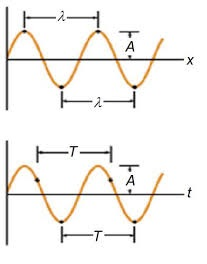
\includegraphics[scale=1]{hull_hossz.jpg}
\caption{Egy hullámon azonos fázisú pontok távolsága (felső ábra), \\és egy tömegpont kitérése az idő függvényében (alsó ábra).}
\end{figure}

A hullámokat több szempont szerint is csoportosíthatjuk. Egyrészt a közeg kiterjedtsége szempontjából lehet egy hullám 1 dimenziós (pl.\ kifeszített kötélen), 2 dimenziós (pl.\ víz felszínén) vagy 3 dimenziós (pl.\ a hang), másrészt a tömegpontok kitérése alapján lehet egy hullám longitudinális vagy transzverzális, ahol a tömegpontok kitérése és a hullám terjedési iránya rendere párhuzamos, illetve merőleges.

% ----------------------------------------------------------------
\subsection{Állóhullámok}

A tapasztalat szerint egy hullám vissza tud verődni, ha egy másik közeggel találkozik. A két közegtől függően ez lehet teljes visszaverődés vagy részleges visszaverődés is. A visszaverődést matematikailag úgy tudjuk leírni, hogy két irányba terjed egy-egy hullám, amiknek különböző hullámfüggvényük van,
$$ \Psi(x, t) = \Psi_{\rightarrow}(x, t) + \Psi_{\leftarrow}(x, t) = A^\prime \cdot \sin(\omega t - k x + \varphi) - A^{\prime \prime} \cdot \sin(\omega t + k x + \varphi^\prime). $$
A teljes visszaverődés esetét véve, azaz $A^\prime = A^{\prime \prime}$, a különbség átírható a
$$ \Psi(x, t) = A \sin(k x + \beta) \cos(\omega t + \alpha) $$
alakba. Ebből a képletből lehet leginkább látni hogy az idő és a hely függés két külön tagban szerepel aminek eredménye az, hogy a hullám látszólag nem mozog, tehát pontjai egy adott helyen mindig azonos amplitúdóval rezegnek.

Egy mindkét végén rögzített húr esetét nézve két kényszert tudunk felírni. Az $L$ hosszú húr szélein a kitérés mindig $0$ kell legyen, így $\Psi(0, t) = \Psi(L, t) = 0$. Ezt beírva $\beta = 0$ adódik, illetve a $\sin(k L) = 0$, azaz $k L = n \pi$ kényszer, ahol $n = \text{1, 2, 3, ...}$ . Ezzel a hullámhosszra és a körfrekvenciára további kényszereket kapunk,
$$ \lambda_n = \frac{2 \pi}{k} = \dfrac{2 L}{n}, $$
$$ \omega_n = k c = \frac{n \pi c}{L}, \quad f_n = \frac{\pi c}{2 L}. $$
Azt látjuk, hogy a rezgés frekvenciája csak az $f_1$ alapfrekvencia egész számú többszöröse lehet. Ezeket felharmonikusoknak nevezzük.

\begin{figure}[h!]
\centering
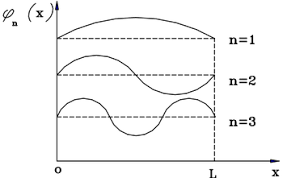
\includegraphics[width=7cm]{allohullam.png}
\caption{Különböző állóhullámok húron. \cite{mintamuszer}}
\end{figure}

%-----------------------------------------------------------------
\subsection{Hanghullámok}

A hang az egyik leggyakoribb hullám a természetben. Ennek a hullámnak fizikai tulajdonságait vizsgálva egy longitudinális mechanikai gömbhullámról van szó, ez azt jelenti hogy ha egy pontszerű forrásból indul a regés akkor gömb alakú hullámfrontok keletkeznek és a deformáció iránya azonos a terjedési iránnyal. A hang, mint minden mechanikai hullám csak közegben tud terjedni, ami a mi esetünkben általában levegő, de vízben például vízben is ugyanúgy tud terjedni. Hanghullámok keltése bármilyen olyan rezgéssel lehetséges mely zavart visz a közegbe. Sokszor szokás a hangokat felerősíteni, főleg hangszereknél, úgynevezett rezonátorokkal. Ezek általában üreges fa testek szoktak lenni. Ezeket a hanghullám gerjeszti, így a rezonanciafrekvenciáihoz közeli hangokat felerősíti.

% ----------------------------------------------------------------
\subsection{Fourier transzformáció}

A Fourier transzformáció egy matematikai művelet mely egy $F(t)$ időtérbeli függvényt egy $f(\omega)$ frekvenciatérbeli függvénnyé transzformál. Ennek a műveletnek az alapjait a Fourier sorfejtés elvében találjuk mely szerint bármilyen periodikus jelet harmonikus jelek összegére fel lehet bontani, tehát bármilyen periodikus jelet felírhatunk mint szinuszok és koszinuszok összege. Ennek egy általánosítása a Fourier transzformáció mely bármilyen aperiodikus jelre alkalmazható,
$$ f(\omega) = \frac{1}{\sqrt{2\pi}} \int^{\infty}_{-\infty} F(t) \cdot e^{i \omega t} \D t. $$
Az időtérbe való visszatéréshez az inverz Fourier transzformáció
$$ F(t) = \frac{1}{\sqrt{2\pi}} \int^{\infty}_{-\infty} f(\omega) \cdot e^{-i \omega t} \D \omega. $$

Ennek elvégzésére a leggyakoribb algoritmus az úgynevezett \emph{Fast Fourier Transform} (FFT). Sok helyzetben egyszerűbb frekvenciatérben dolgozni, így ezt a fizika sok területén alkalmazzák. Vegyünk például egy tisztán szinuszos jelet ami egy adott $f$ frekvenciával változik, ha ennek a jelnek vesszük a Fourier transzformáltját egy olyan függvényt kapunk mely mindenhol nulla kivéve az $f$ frekvencia helyén.

\begin{figure}[!h]
\centering
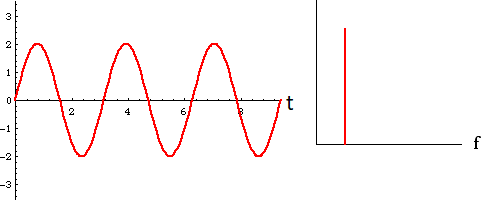
\includegraphics[scale=1]{PowerSpectrum1.png}
\caption{$2 \sin(\omega t)$ (bal), Fourier transzformált (jobb)}
\end{figure} 

Az általunk végzett kísérletben hanghullámokat vizsgálunk melyek általában nem tisztán harmonikusan rezegnek, hanem mindig több, különböző frekvenciájú, harmonikus jelek keverednek. Ezek a jelek más-más intenzitással jelennek meg és ha minden komponensnek a járulékát szeretnénk látni, akkor Fourier transzformációt kell alkalmaznunk, hogy felbonthassuk a jelet. A transzformált jel amplitúdó - frekvencia grafikonját hívjuk spektrumnak.

% ----------------------------------------------------------------
\subsection{Hullámterjedés megfeszített rugalmas húron}

A \ref{hur_hullam}.\ ábrán egy megfeszített rugalmas húr kicsiny darabjáról látunk egy ábrát. A hullám az $x$-tengely mentén terjed, a húr kitérése $y$ irányú és a húrt $\V{T}(x, t)$ erő feszíti. Ezen kívül felvettük a feszítőerő $x$-tengellyel bezárt $\alpha(x, t)$ szögét.

\begin{figure}[!h]
\centering
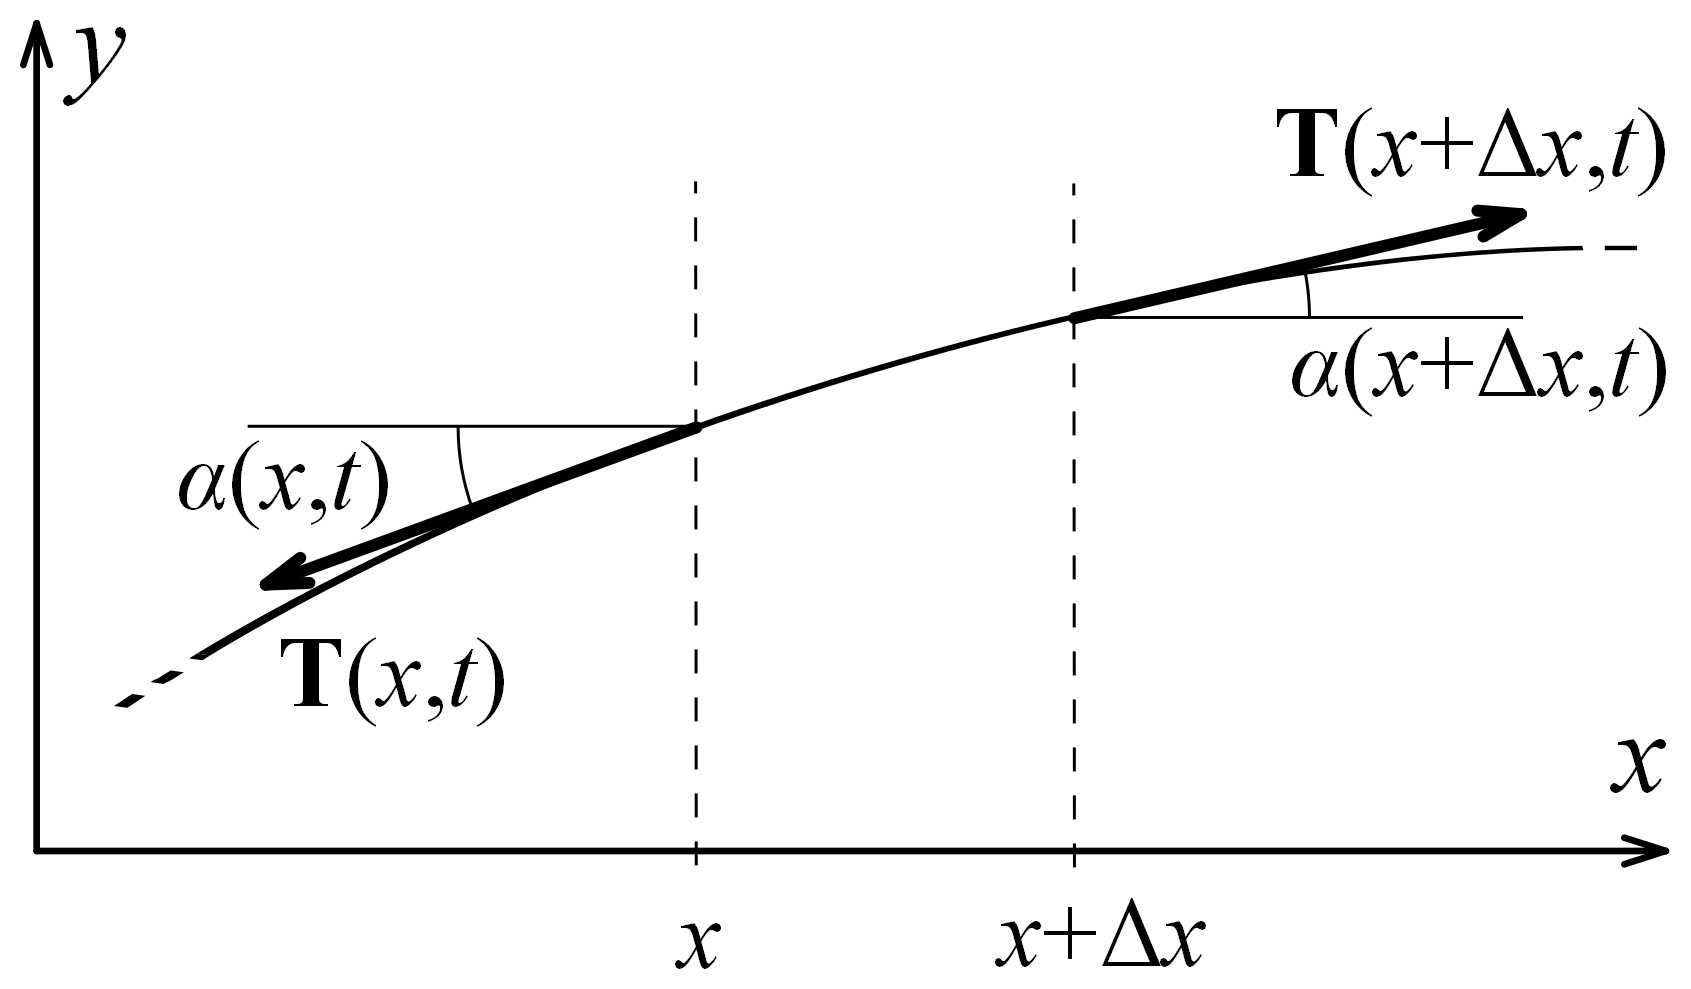
\includegraphics[width = 10cm]{hur_hullam.png}
\caption{Hullám terjedése megfeszített rugalmas húron. \cite{kisfiz1}}
\label{hur_hullam}
\end{figure}

A húrdarabra felírthatjuk a mozgásegyenletet,
$$ \Delta F_y = \Delta m a_y, $$
ahol az $y$ irányú erő
$$ \Delta F_y = T_y(x + \Delta x, t) - T_y(x, t) = $$
$$ = T(x + \Delta x, t) \cdot \sin\alpha(x + \Delta x, t) - T(x, t) \cdot \sin\alpha(x, t). $$
Felhasználva, hogy $T(x, t) \approx T = \text{állandó}$ és $\alpha(x, t) \ll 1$
$$ \Delta F_y = T \left[ \tg\alpha(x + \Delta x, t) - \tg\alpha(x, t) \right] \approx T \frac{\partial \tg\alpha(x, t)}{\partial x} \Delta x $$
adódik. Továbbá felhasználva, hogy
$$ \tg\alpha(x, t) = \frac{\partial \Psi(x, t)}{\partial x} \quad \text{és} \quad a_y = \frac{\partial^2 \Psi(x, t)}{\partial t^2} $$
a mozgásegyenlet felírható
$$ T \frac{\partial^2 \Psi(x, t)}{\partial x^2} = \frac{\Delta m}{\Delta x} \frac{\partial^2 \Psi(x, t)}{\partial t^2} $$
alakban. Ezt összevetve az hullámegyenlet \eqref{hullamegyenlet-1D} képletével a hullám terjedési sebességére
$$ c = \sqrt{\frac{T}{\mu}} $$
adódik, ahol $\mu = \frac{\Delta m}{\Delta x}$ a lineáris tömegsűrűség.



% ================================================================
\section{Spektrumanalizátor program}

A mérésünk nem igényel bonyolult kapcsolásokat vagy számolásokat a lementett adatokkal és ez nagyrészt a hozzá írt Labview és C++ programoknak \cite{github} köszönhető. A program elindításához nyissuk meg a \texttt{spectrum\_analysis.lvproject} fájlt a \emph{LabView NXG 1.0} programmal. Ezután a programban felül a \texttt{Library.sli} fülre menve meg kell adni a projekttel mellékelt, annak mappájában lévő \texttt{frequency\_peaks.dll} fájl helyét.

Ezután a mérés elkezdéséhez nincs más dolgunk mint csatlakoztatni a myDAQ-ot a számítógépünkhöz, az \textit{audio in} bemenetre egy mikrofont kapcsolni, majd a programot elindítva elkezdhetjük a mérést.

A program a myDAQ-hoz csatlakoztatott mikrofonnal egy adott hosszúságú ideig mérést végez. Ezután a mért adatoknak spektrum analízisét hajtja végre. A mérés elindítása után a \ref{labview}.\ ábrához hasonló képet kell látnunk.

\begin{figure}[h]
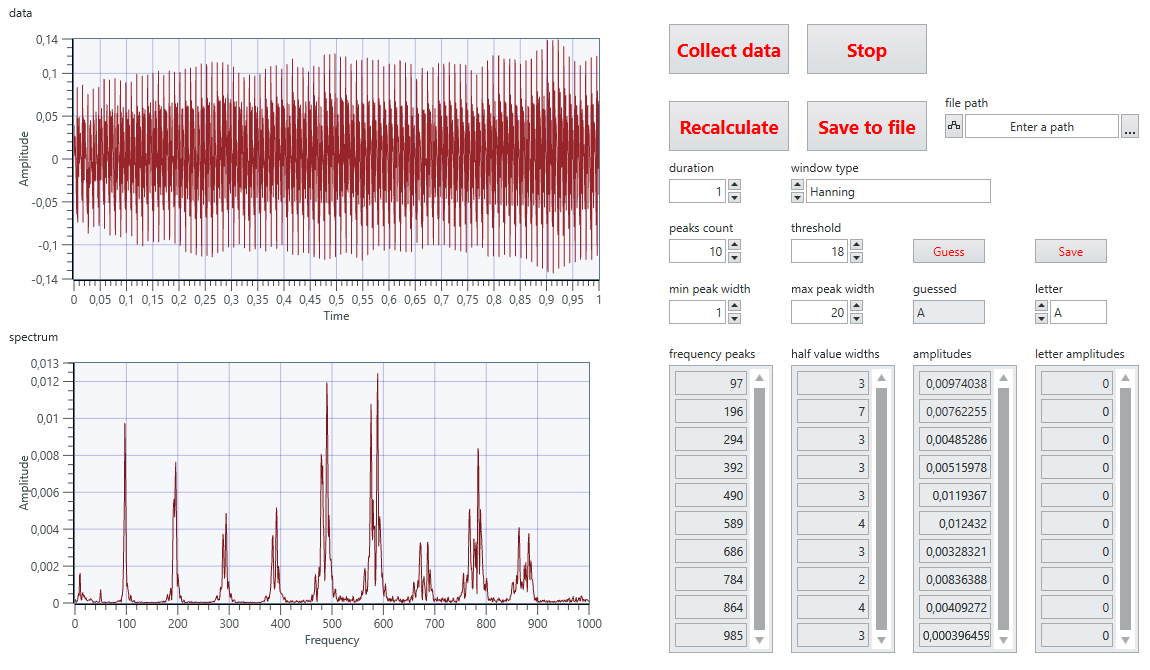
\includegraphics[width=\textwidth]{labview.png}
\caption{}
\label{labview}
\end{figure}

Az ablakban két grafikon van, a felső a mért adatok, az alsó annak a Fourier transzformációja. A programban négy fontos gomb található,
\begin{itemize}
\item \emph{Collect data}, ez indítja el az adatok gyűjtését, annyi másodpercig mér, amennyi a \emph{duration} mezőben meg van adva,
\item \emph{Stop}, ez leállítja a mérést,
\item \emph{Recalculate}, ezzel újra lehet ugyanarra az adatokra számítani a Fourier transzformációt és a csúcsokat. Ez a gomb akkor hasznos, ha a program nem találja meg egyből a csúcsokat a beállított paraméterekkel, vagy rossz ablakot állítottunk be a Fourier transzformációhoz,
\item \emph{Save to file}, ez elmenti a talált csúcsokat a \emph{file path} mezőben megadott fájlba. Ezt szöveges formátumban teszi meg és a fájl végére írja az adatokat, így a korábban mentett adatokat nem írja felül.
\end{itemize}
Még kívül 7 paramétert állíthatunk,
\begin{itemize}
\item \emph{duration} a mérés időtartama másodperben,
\item \emph{peaks count} a keresett csúcsok száma,
\item \emph{threshold} a keresett csúcsok minimális magassága dB-ben,
\item \emph{min peak width}, \emph{max peak widht} a keresett csúcsok minimális és maximális szélessége Hz-ben,
\item \emph{file path} az a fájl, ahova a \emph{Save to file} gomb elmenti az adatokat,
\item \emph{window tipe} a Fourier transzformációhoz használt ablakfüggvény. Alapvetően a \emph{Flat top} és \emph{Hanning} ablakokat használjuk, ezek rendre a pontos amplitúdó és a pontos frekvencia méréséhez használhatóak.
\end{itemize}

A program által talált frekvenciacsúcsok adatait a \emph{frequency peaks}, a \emph{half value widths} és az \emph{amplitudes} táblázatokból tudjuk leolvasni. Ezek rendre a frekvenciacsúcsok helyei Hz-ben, a frekvenciacsúcsok félértékszélessége Hz-ben és a frekvenciacsúcsok amplitúdói V-ban.

A \emph{magánhangzók spektrumának vizsgálata} méréshez ezen kívül még használjuk a \emph{Save} gombot, ami a \emph{letter} mezőben megadott betűhöz rendeli a legutóbbi mérésből származó frekvenciacsúcsok értékeit. Ha az összes magánhangzóhoz elmentettük a frekvenciacsúcsok nagyságát, akkor egy új felvételt készíthetünk, és ezután a \emph{Guess} gombra kattintva a program megpróbálja kitalálni, hogy milyen magánhangzót mondtunk ki ebben a mérésben, amit az alatta lévő \emph{guessed} ablakban láthatunk.



% ================================================================
\section{Magánhangzók spektrumának vizsgálata}

Az emberi kommunikációnak a legalapvetőbb formája a beszéd ami sok évezredeken át fejlődött az és változott az emberek igényei és kultúrájuk szerint. Az embereknek ezen képessége nemcsak a hangszálaknak köszönhető hanem kiemelkedő agyi képességeiknek is. Egy adott szó kiejtése egy összetett folyamat, melynek során a tüdőnkből kiáramló levegő hatására a hangszálaink rezegni kezdenek, így hangot produkálva, amelyet majd a szájüregünk és nyelvünk segítségével modulálunk. Az így generált hangsort az agyunk egy adott tárgyhoz vagy fogalomhoz társítja.

Kísérletünkben csakis a magánhangzók spektrumát vizsgáljuk, mivel ezek úgynevezett tiszta zöngék, amiket úgy keltünk hogy szájüregünket rezonátornak használjuk és ezért több másodpercig is tudjuk őket ``énekelni''. Ezzel szemben a mássalhangzókat ajkunk és nyelvünk mozgatásával keltjük és nem lehet őket folytonosan énekelni ezért nem lehet érdemben a spektrumukat vizsgálni.

Visszatérve a magánhangzókra azt mondtuk hogy a szánk rezonátorként működik a kiejtésüknél, de pontosan mit is jelent ez? Biztosan mindenki próbálta már azt csinálni, hogy egy felfújt lufinak a száját megfeszítve azt megszólaltatta. Ilyenkor a levegő kiáramlik a lufiból és minél feszesebben tartjuk a száját annál magasabb lesz a hang. Testünk hasonlóan működik csak a lufi szerepét a tüdőnk a ``száj'' szerepét pedig a hangszálak játsszák. Aztán az így kialakult hang a torkunkon és szánkon keresztül terjed ahol folyton visszaverődik ezeknek falairól és így sok hanghullám szuperpozícióját halljuk. Minden egyes kombináció más-más végeredményt produkál. A magyar nyelvben 9 magánhangzót különböztetünk meg.

% ----------------------------------------------------------------
\subsection{Mérés menete}

Mérésünk során a 9 magánhangzó (a, á, e, é, o, ö, u, ü) Fourier spektrumát vizsgáltuk három különböző emberrel, annak reményében hogy hasonlóságokat tapasztalunk a hangokban. Az adatgyűjtést a myDAQ mérőkártyával és a hozzá írt Labview programmal végeztük, a mérés menete nem túl bonyolult, elég a mérőkártyához egy mikrofont kapcsolni és a program elindítása után a magánhangzókat egyesével kiejteni és az eredményeket egy fájlba lementeni. Minden hangot háromszor mértünk. Kiemelten fontos az hogy hangosan ejtsük ki a hangokat és ha laptopról mérünk, akkor az ne legyen töltőn. Ennek oka az hogy a mérőkártya a hangerősség mérést feszültségmérésre vezeti vissza és ebben jelen van egy nem elhanyagolható 50 Hz-es zaj, ami a hálózatból ered. Ez önmagában nem jelentene problémát, de ennek felharmonikusai is megjelennek, amik már jelentős hibát okozhatnak a mérésben, mert ezek az emberi beszéd frekvenciatartományában vannak már.

A Fourier transzformációhoz érdemes a \emph{Flat top} ablakot használni, mert ennél a legjobb a csúcsok amplitúdópontossága.

A program által lementett adatokban az amplitúdóértékek normálva vannak a legmagasabb csúcshoz képest, így azokat csak ábrázolni kell már csak.

Ennél a mérésnél a program ki is tudja találni, hogy milyen hangot mond az ember, ha előtte az összes magánhangzóhoz elmentettünk egy-egy mintát. Erről az előző részben beszéltünk részletesebben.

A mérést kevesebb, mint $10$ perc alatt el lehet végezni, a kiértékelés legfeljebb $15$ percet vesz igénybe.

% ----------------------------------------------------------------
\subsection{Mérési eredmények}

\begin{figure}[h]
\centering
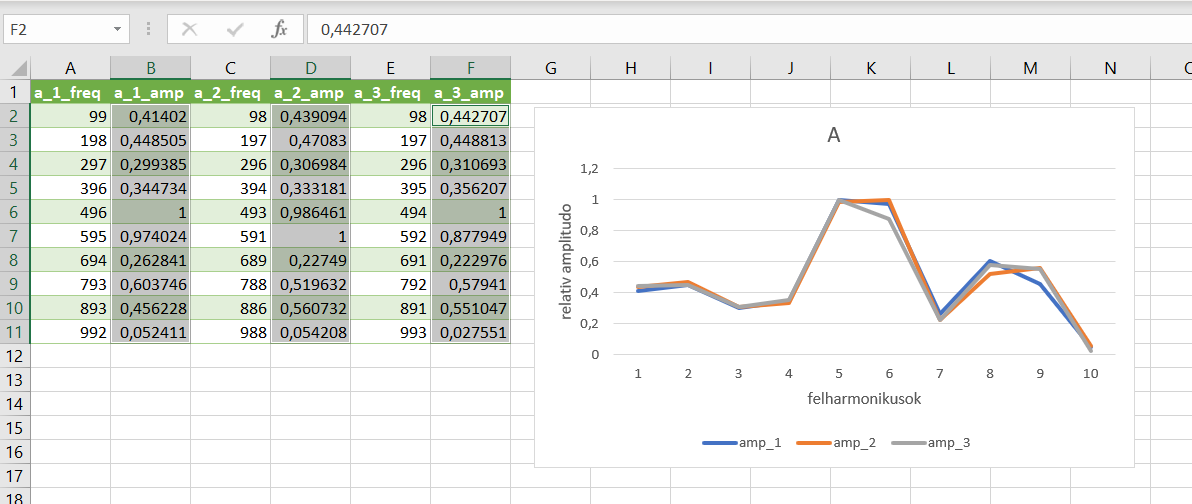
\includegraphics[width=\textwidth]{minta.png}
\caption{Kijelölt rész az ábrázolandó.}
\label{1ábra}
\end{figure}

A \ref{1ábra}.\ ábrán lévő táblázatokból látható hogy a spektrumban megjelenő frekvenciák tényleg az első (alapfrekvencia) egész számú többszörösei. Ha összegyűjtjük minden hang alapfrekvenciáját egy táblázatba, azt tapasztaljuk hogy ezek nagyon közel állnak egymáshoz ha egy alanynak a hangjait vizsgáljuk, viszont eltérnek az alanyok között. Ezt a \ref{1tábla}.\ táblázatban láthatjuk.

\begin{table}[h]
\centering
\begin{tabular}{c|c|c|c}
 & Csanád (Hz) & Zeno (Hz) & Lukács (Hz) \\ 
\hline 
A & 98 & 108 & 137 \\ 
Á & 101 & 114 & 133 \\ 
E & 106 & 110 & 147 \\ 
É & 107 & 113 & 146 \\ 
I & 113 & 152 & 148 \\ 
O & 114 & 119 & 182 \\ 
Ő & 114 & 123 & 197 \\ 
U & 126 & 110 & 183 \\ 
Ű & 128 & 155 & 159 \\ 

\end{tabular} 
\caption{Alapfrekvenciák átlagértékei minden betűre.}
\label{1tábla}
\end{table}  

Mivel a különböző hangok alapfrekvenciái nagyjából azonosak egy adott embernél és az ugyanolyan hangok alapfrekvenciái mások különböző embereknél, a hangok között a felharmonikusok arányában lehet csak különbség. Azokat ábrázolva láthatjuk, hogy mi különbözteti meg a magánhangzókat egymástól. Ezt a \ref{o_felharmonikusok}.\ ábrán láthatjuk.

\begin{figure}[h!]
\centering
\begin{subfigure}[t]{.5\linewidth}
\centering
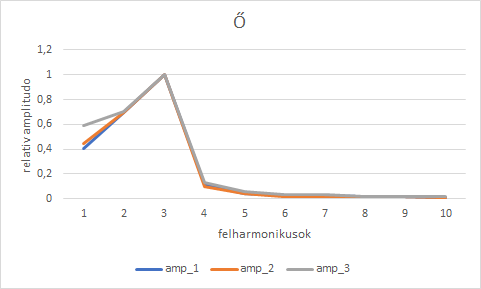
\includegraphics[width = \linewidth]{csanad_o.png}
\caption{Csanád ``Ö'' hangjának felharmonikusainak aránya.}
\end{subfigure}%
\begin{subfigure}[t]{.5\linewidth}
\centering
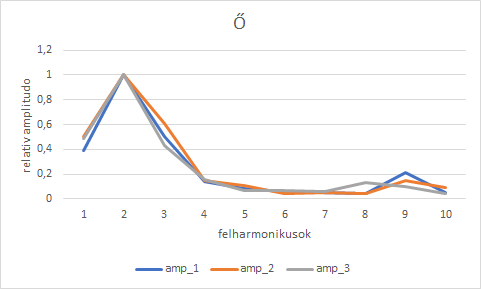
\includegraphics[width = \linewidth]{lukacs_o.png}
\caption{Lukács ``Ö'' hangjának felharmonikusainak aránya.}
\end{subfigure}
\begin{subfigure}[t]{.5\linewidth}
\centering
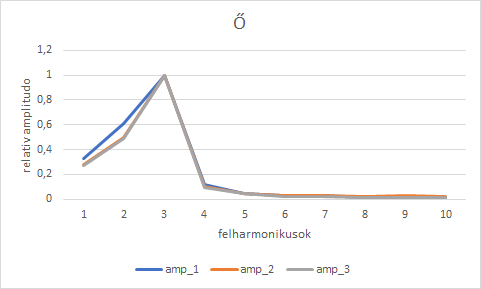
\includegraphics[width = \linewidth]{zeno_o.png}
\caption{Zeno ``Ö'' hangjának felharmonikusainak aránya.}
\end{subfigure}
\caption{}
\label{o_felharmonikusok}
\end{figure}

Ezekből tisztán látható az hogy az ``Ö'' hangnak a második vagy a harmadik felharmonikusa a legerősebb, az előtte lévők valamivel gyengébbek, míg a többi gyakorlatilag elhanyagolható hozzájuk képest. A többi hangot is ábrázolhatjuk, ezt a \ref{a_a}-\ref{u_u}.\ ábrákon láthatjuk.

\begin{figure}[h!]
\begin{subfigure}[t]{.5\linewidth}
\centering
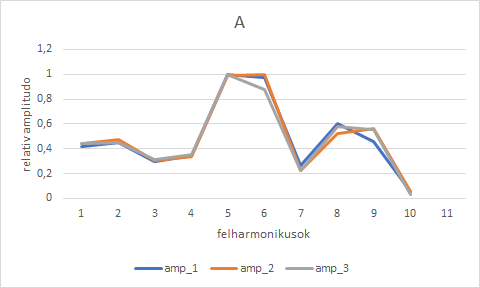
\includegraphics[width = \linewidth]{A.png}
\end{subfigure}%
\begin{subfigure}[t]{.5\linewidth}
\centering
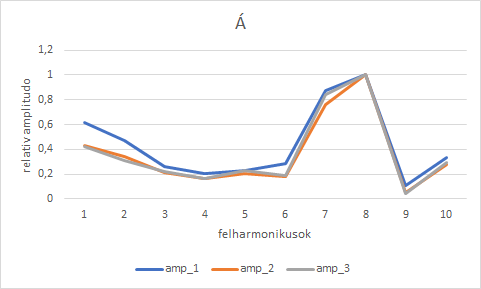
\includegraphics[width = \linewidth]{A_1.png}
\end{subfigure}
\caption{``A'' és ``Á'' hangok.}
\label{a_a}
\end{figure}

\begin{figure}[h!]
\begin{subfigure}[t]{.5\linewidth}
\centering
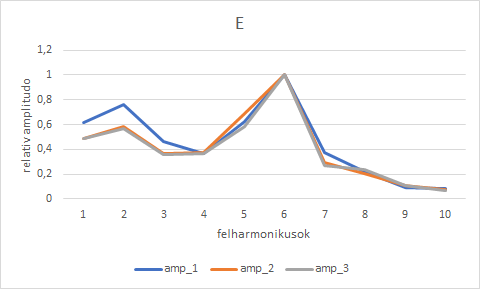
\includegraphics[width = \linewidth]{E.png}
\end{subfigure}%
\begin{subfigure}[t]{.5\linewidth}
\centering
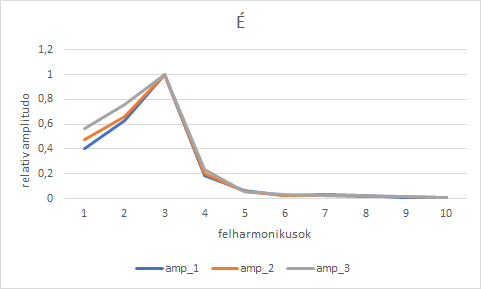
\includegraphics[width = \linewidth]{E_1.png}
\end{subfigure}
\caption{``E'' és ``É'' hangok.}
\label{e_e}
\end{figure}

\begin{figure}[h!]
\begin{subfigure}[t]{.5\linewidth}
\centering
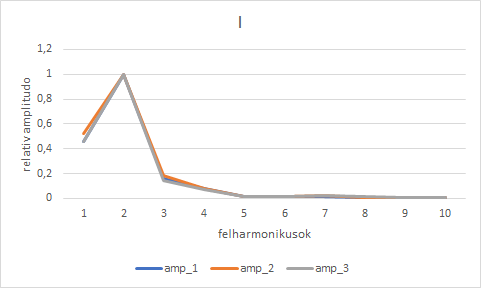
\includegraphics[width = \linewidth]{I.png}
\end{subfigure}%
\begin{subfigure}[t]{.5\linewidth}
\centering
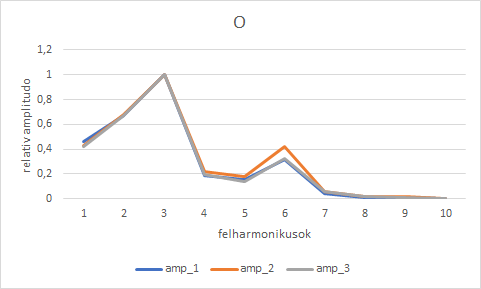
\includegraphics[width = \linewidth]{O.png}
\end{subfigure}
\caption{``I'' és ``O'' hangok.}
\label{i_o}
\end{figure}

\begin{figure}[h!]
\begin{subfigure}[t]{.5\linewidth}
\centering
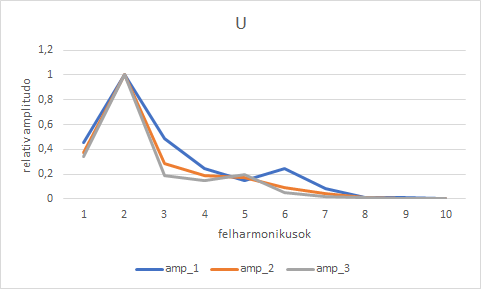
\includegraphics[width = \linewidth]{U.png}
\end{subfigure}%
\begin{subfigure}[t]{.5\linewidth}
\centering
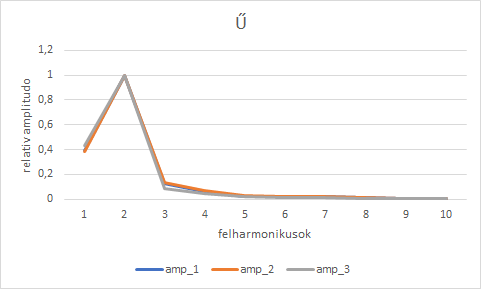
\includegraphics[width = \linewidth]{U_1.png}
\end{subfigure}
\caption{``U'' és ``Ü'' hangok.}
\label{u_u}
\end{figure}

A felharmonikusok arányát nézve azt látjuk, hogy szinte az összes magánhangzó egyedi. Legjobban az ``I'' és ``Ü'', illetve az ``É'' és ``Ö'' hasonlítanak legjobban egymásra. Így ezzel a módszerrel különbséget tudunk tenni a különböző magánhangzók között.




% ================================================================
\section{Húrok frekvencia spektrumának vizsgálata}

Ebben a mérésben neylon hárfahúrokat feszítettünk meg a \ref{muszer_abra}.\ ábrán látható készülék mintájára és mértük a hangjuk alapfrekvenciáját, amiből meghatároztuk a vastagságukat. A mérés maga nagyjából fél óra alatt elvégezhető, ha egy tapasztaltabb ember végzi, kiértékeléssel együtt $45$ percre becsüljük a mérés időtartamát.

% ----------------------------------------------------------------
\subsection{Elméleti összefoglaló}

Egy mindkét végén rögzített húrban a kialakuló állóhullámok alapfrekvenciáját a
$$ f_0 = \frac{c}{2 L} $$
képlet alapján számolhatjuk, ahol $L$ a rögzítési pontok közti távolság. Korábban láttuk, hogy egy megfeszített húrban a hullámterjedési sebességet meghatározhatjuk a $T$ feszítőerő és $\mu$ lineáris tömegsűrűség ismeretében,
$$ c = \sqrt{\frac{T}{\mu}}. $$
Továbbá a húr anyagának $\rho$ térfogati tömegsűrűsége ismeretében a lineáris tömegsűrűség kifejezhető,
$$ \mu = \rho \frac{d^2}{4} \pi, $$
ahol $d$ a húr átmérője. Ezzel az alapfrekvenciára a
$$ f_0 = \frac{1}{d L \sqrt{\rho \pi}} \sqrt{T} $$
képlet adódik.

Egy húrnál az alapfrekvencia és a feszítőerő mérésével így meghatározható annak vastagsága. Ehhez az $f_0$-$T$ összefüggésre egy $f(T) = C \sqrt{T + T_0}$ alakú függvényt illeszthetünk. $C$ kifejezhető,
$$ C = \frac{1}{d L \sqrt{\rho \pi}}, $$
$T_0$ pedig egy konstans tag, ami magába foglalja a feszítő kar súlyából és a súlyok felfüggesztéséhez használt madzag súlyából származó feszítőerőt.

A méréshez mi neylon hárfahúrokat használtunk, viszont akármilyen más, ismert sűrűségű anyagból készült húr is megfelel a célnak, mint például egy acél húr.

% ----------------------------------------------------------------
\subsection{Mérési elrendezés}

\begin{figure}[h!]
\centering
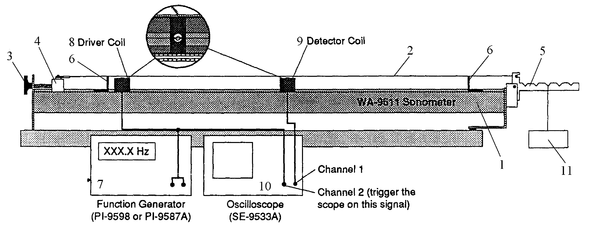
\includegraphics[width =.6\textwidth]{berendezes1.png}
\caption{A mérési berendezés építésének alapjául szolgáló mintakészülék. \cite{mintamuszer}}
\label{muszer_abra}
\end{figure}

\begin{figure}[h!]
\centering
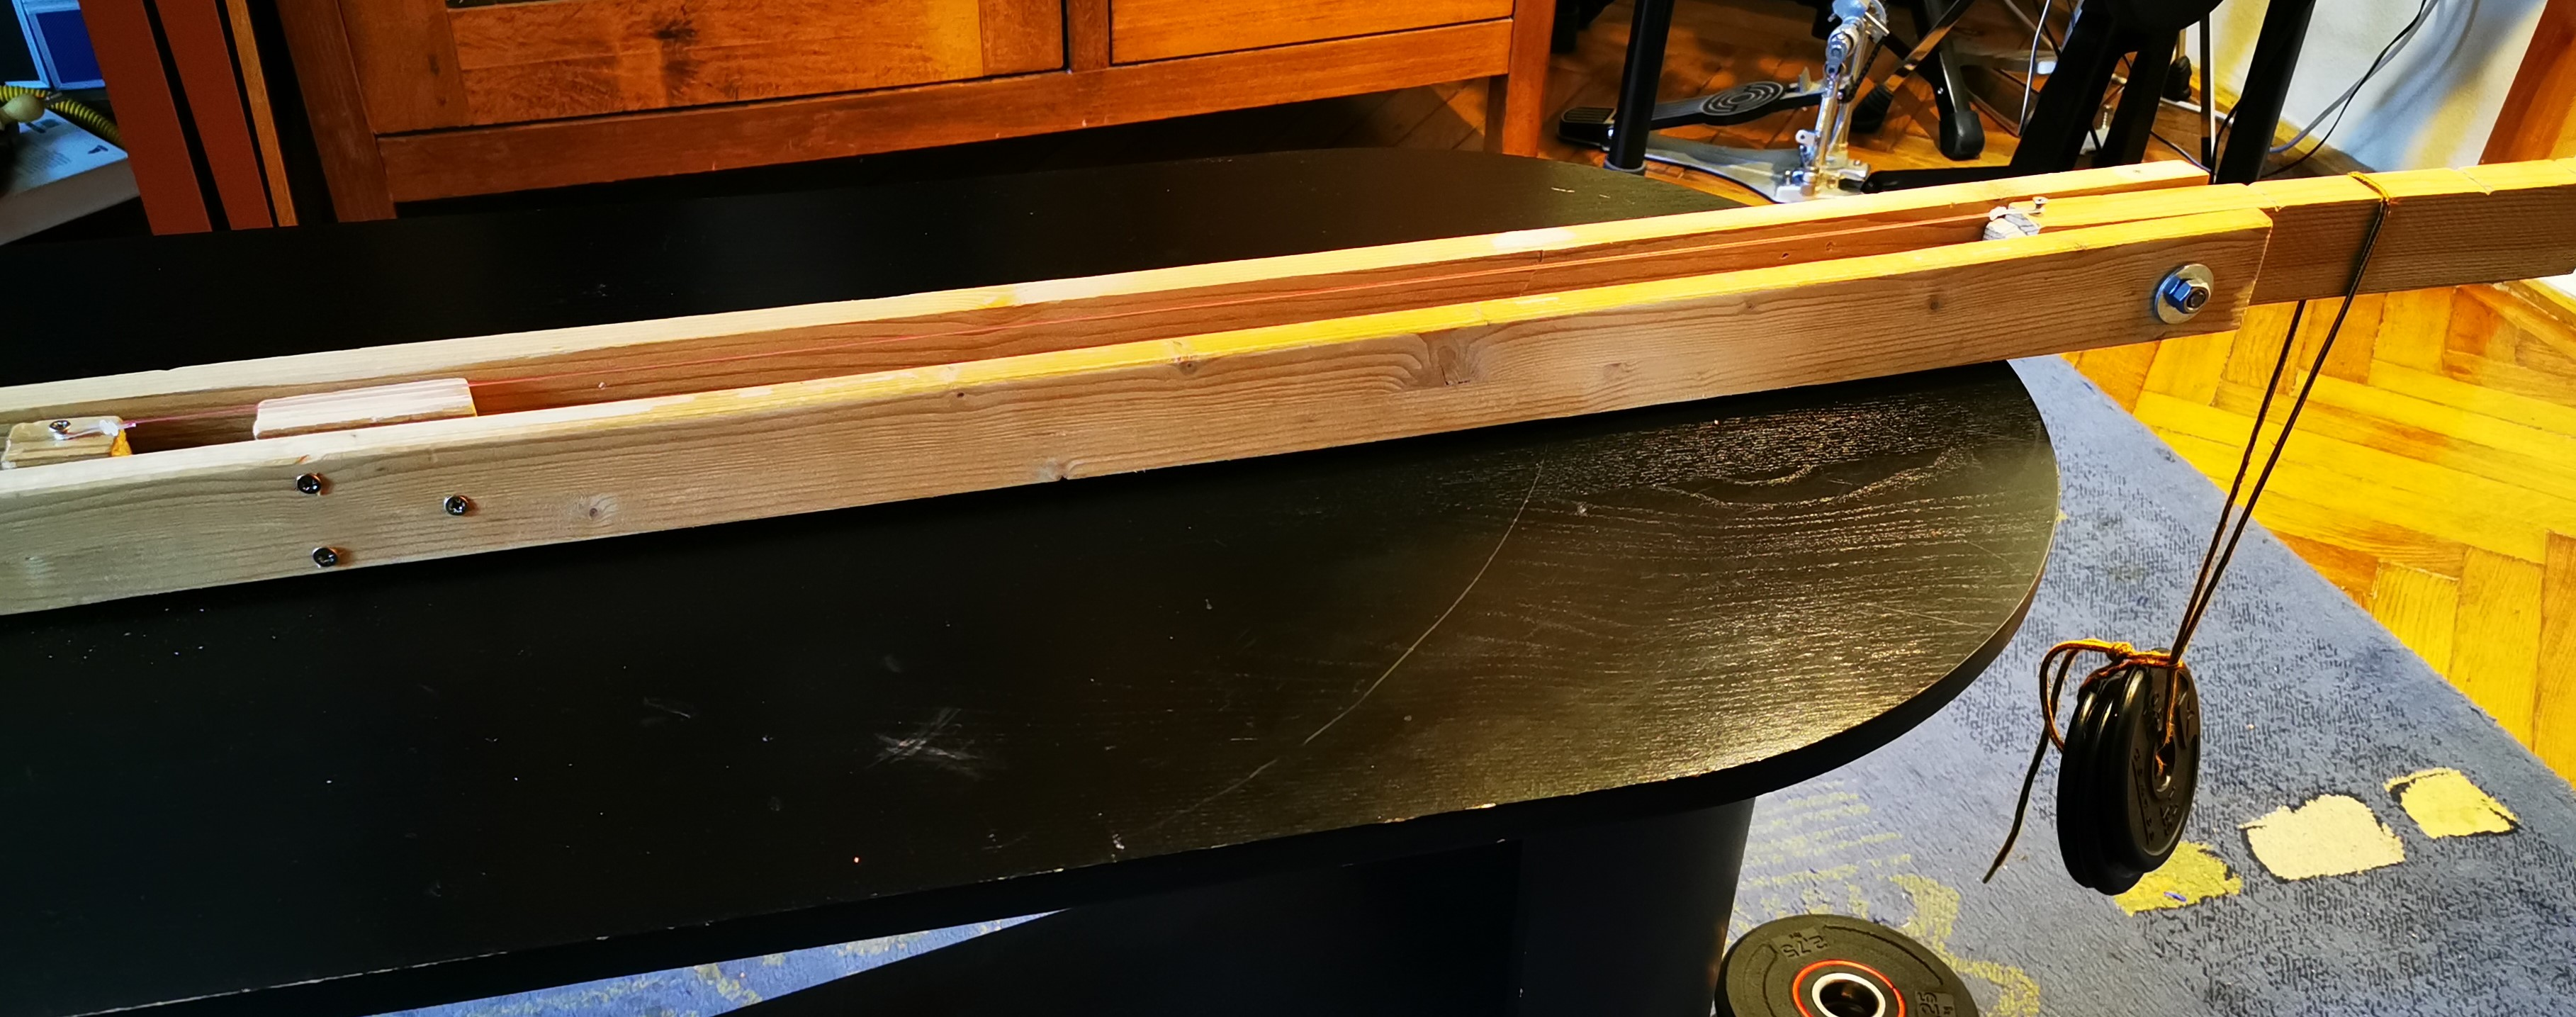
\includegraphics[width = \linewidth]{elejesullyal.jpg}
\caption{A mérőpad.}
\label{muszer}
\end{figure}

A \ref{muszer_abra}.\ ábra mintájára épitettük meg a mérőpadunkat, amit a \ref{muszer}.\ ábrán láthatunk. A pad alapját két párhuzamos farúd alkotja. Az egyik végén a húr egy szabadon forgó rúdra van erősítve, ami nagyjából $20$\,cm-t túl lóg a párhuzamos farudakon. Így ha egy súlyt helyezünk erre az elemre a húrt ismert erővel tudjuk feszíteni. A méréshez ebbe a rúdba $4$ bevágást ejtettünk úgy, hogy a húrt feszítő erő a súlynak rendre $1$, $2$, $3$ és $4$-szerese legyen. Ezt a \ref{erokar}.\ ábrán láthatjuk közelebbről.

\begin{figure}[h!]
\centering
\begin{subfigure}[t]{.4\linewidth}
\centering
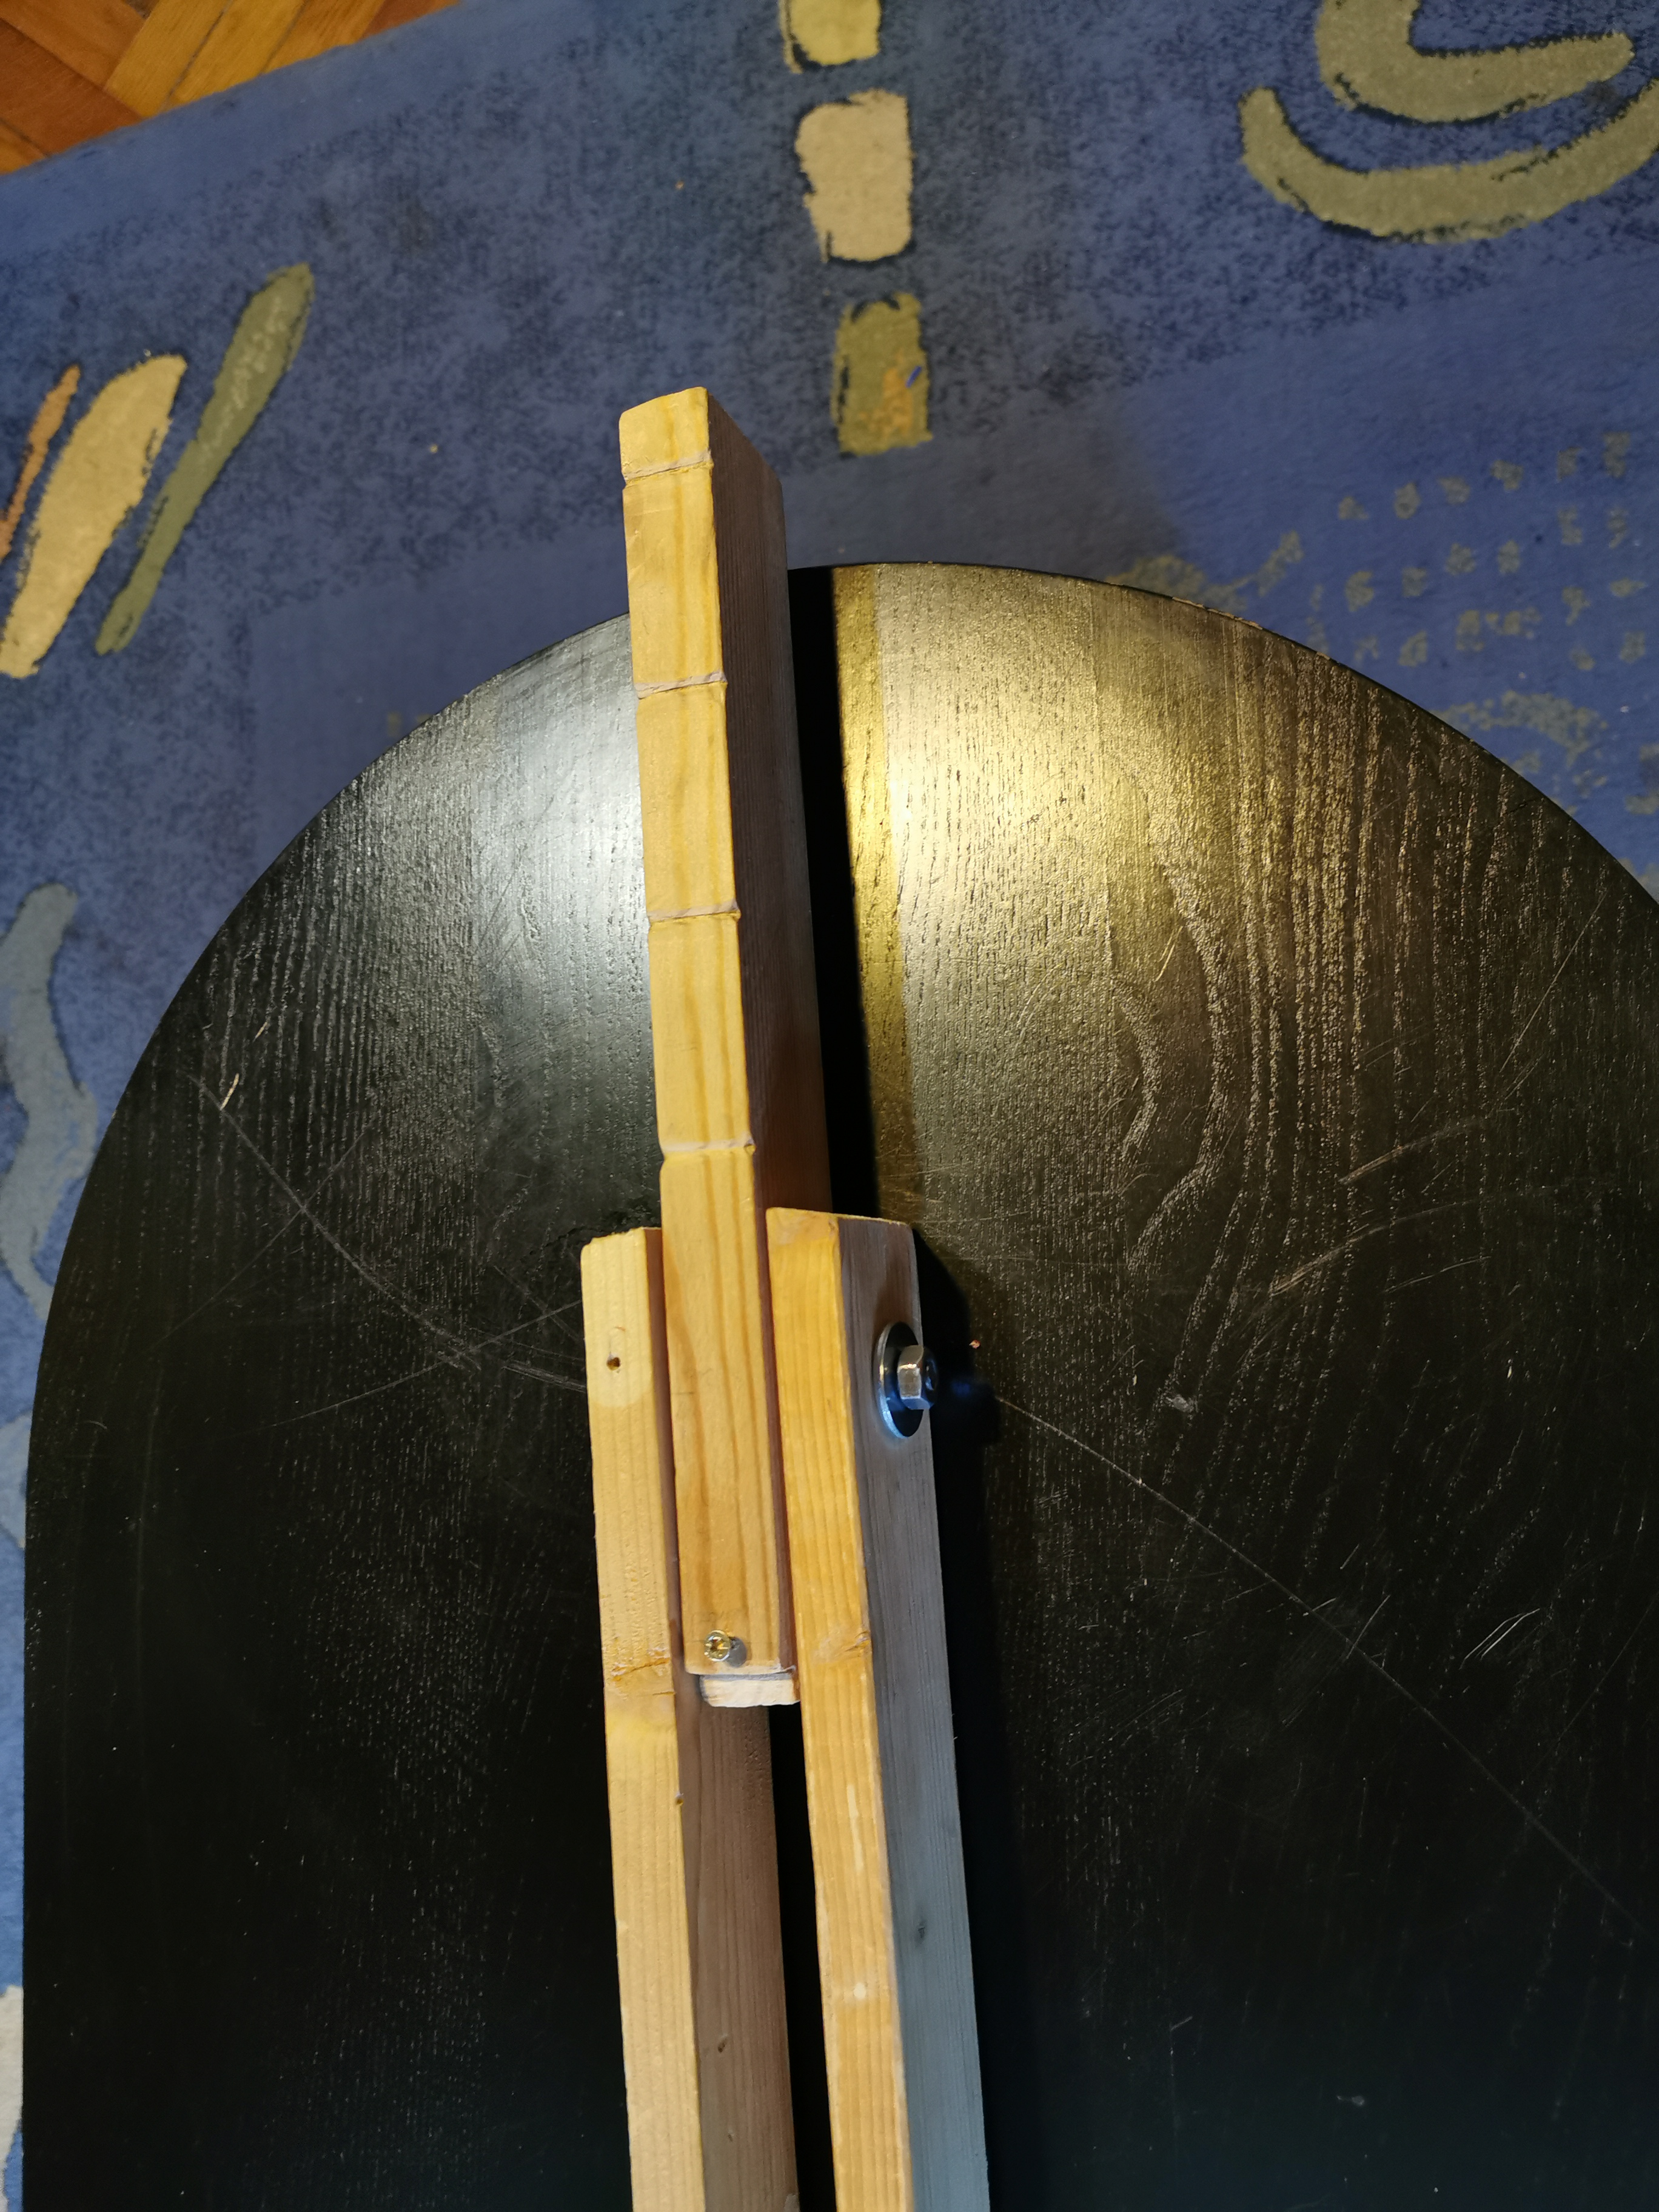
\includegraphics[width=\linewidth]{elejesulynelkul.jpg}
\end{subfigure}%
~~
\begin{subfigure}[t]{.4\linewidth}
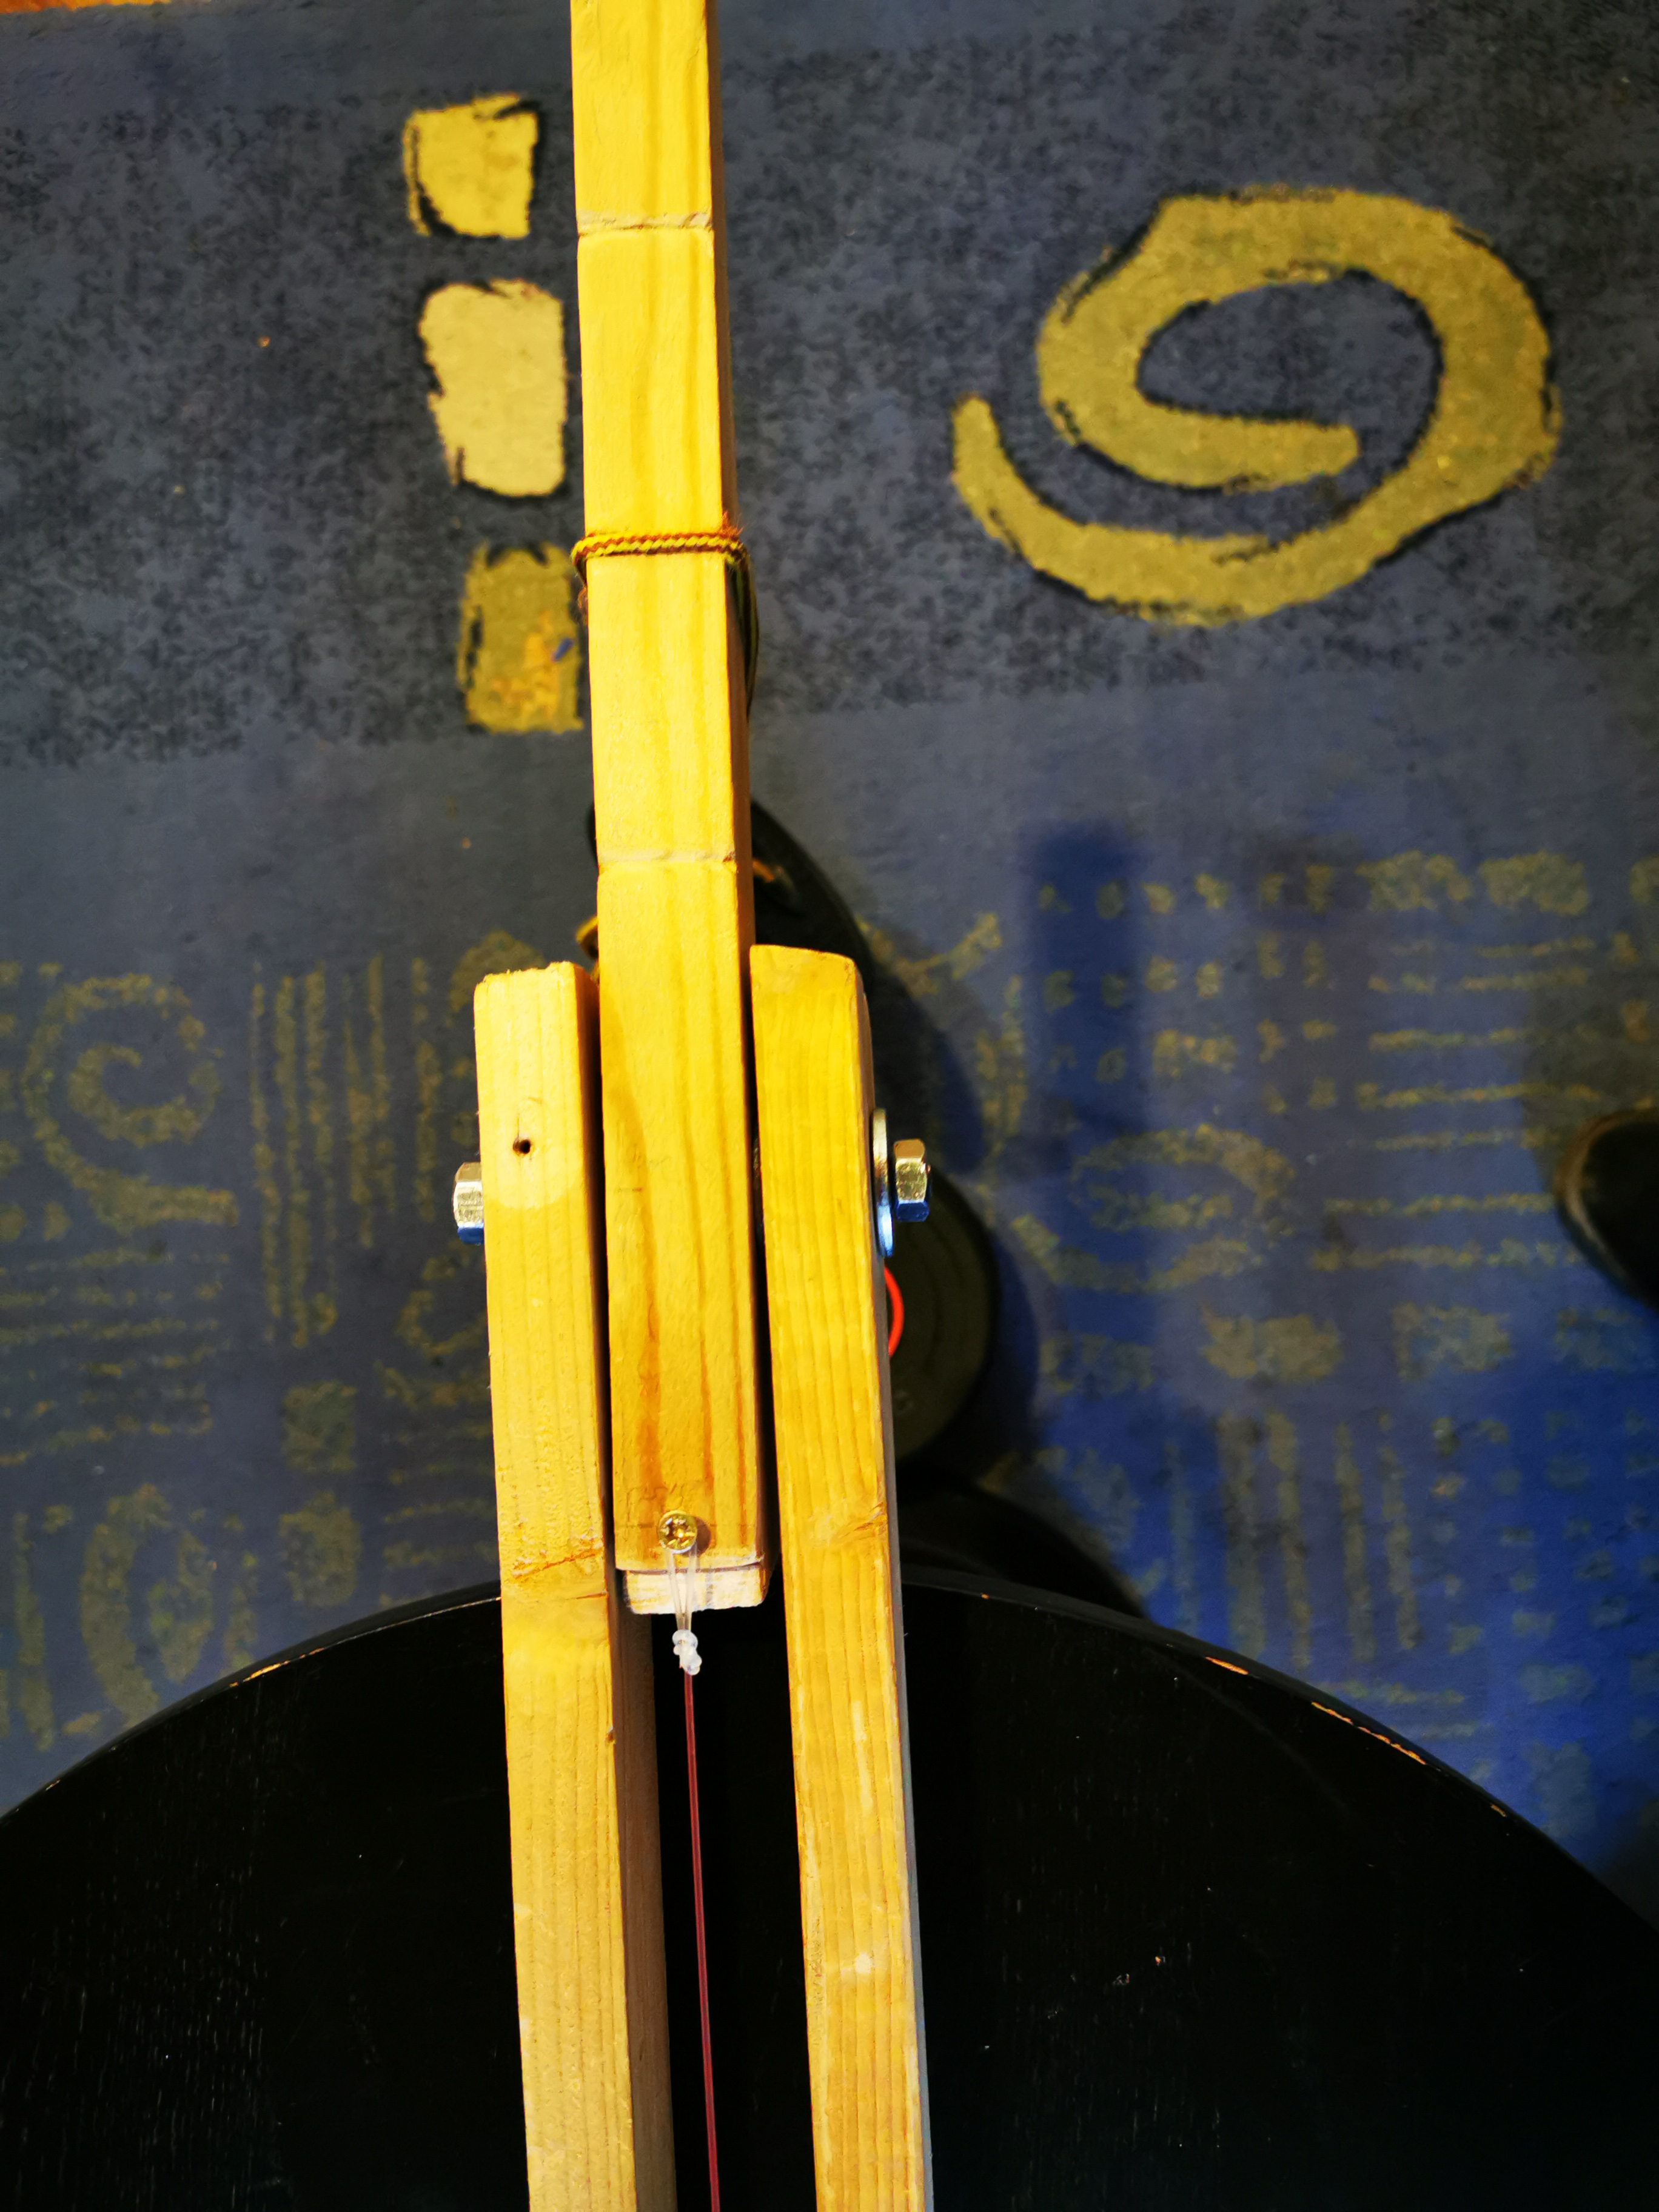
\includegraphics[width=\linewidth]{eleje.jpg}
\end{subfigure}
\caption{A húrt feszítő elem.}
\label{erokar}
\end{figure}

A mérőpad másik végénél két fadarab közé egy menetes szárat erősítettünk. Arra egy másik fadarabot, amin a húr másik vége van rögzítve és egy anyacsavart helyeztünk, így a húr rögzítésének helyét tudjuk mozgatni. Ezt a \ref{menetes}.\ ábrán láthatjuk.

\begin{figure}[h!]
\centering
\begin{subfigure}[t]{.4\linewidth}
\centering
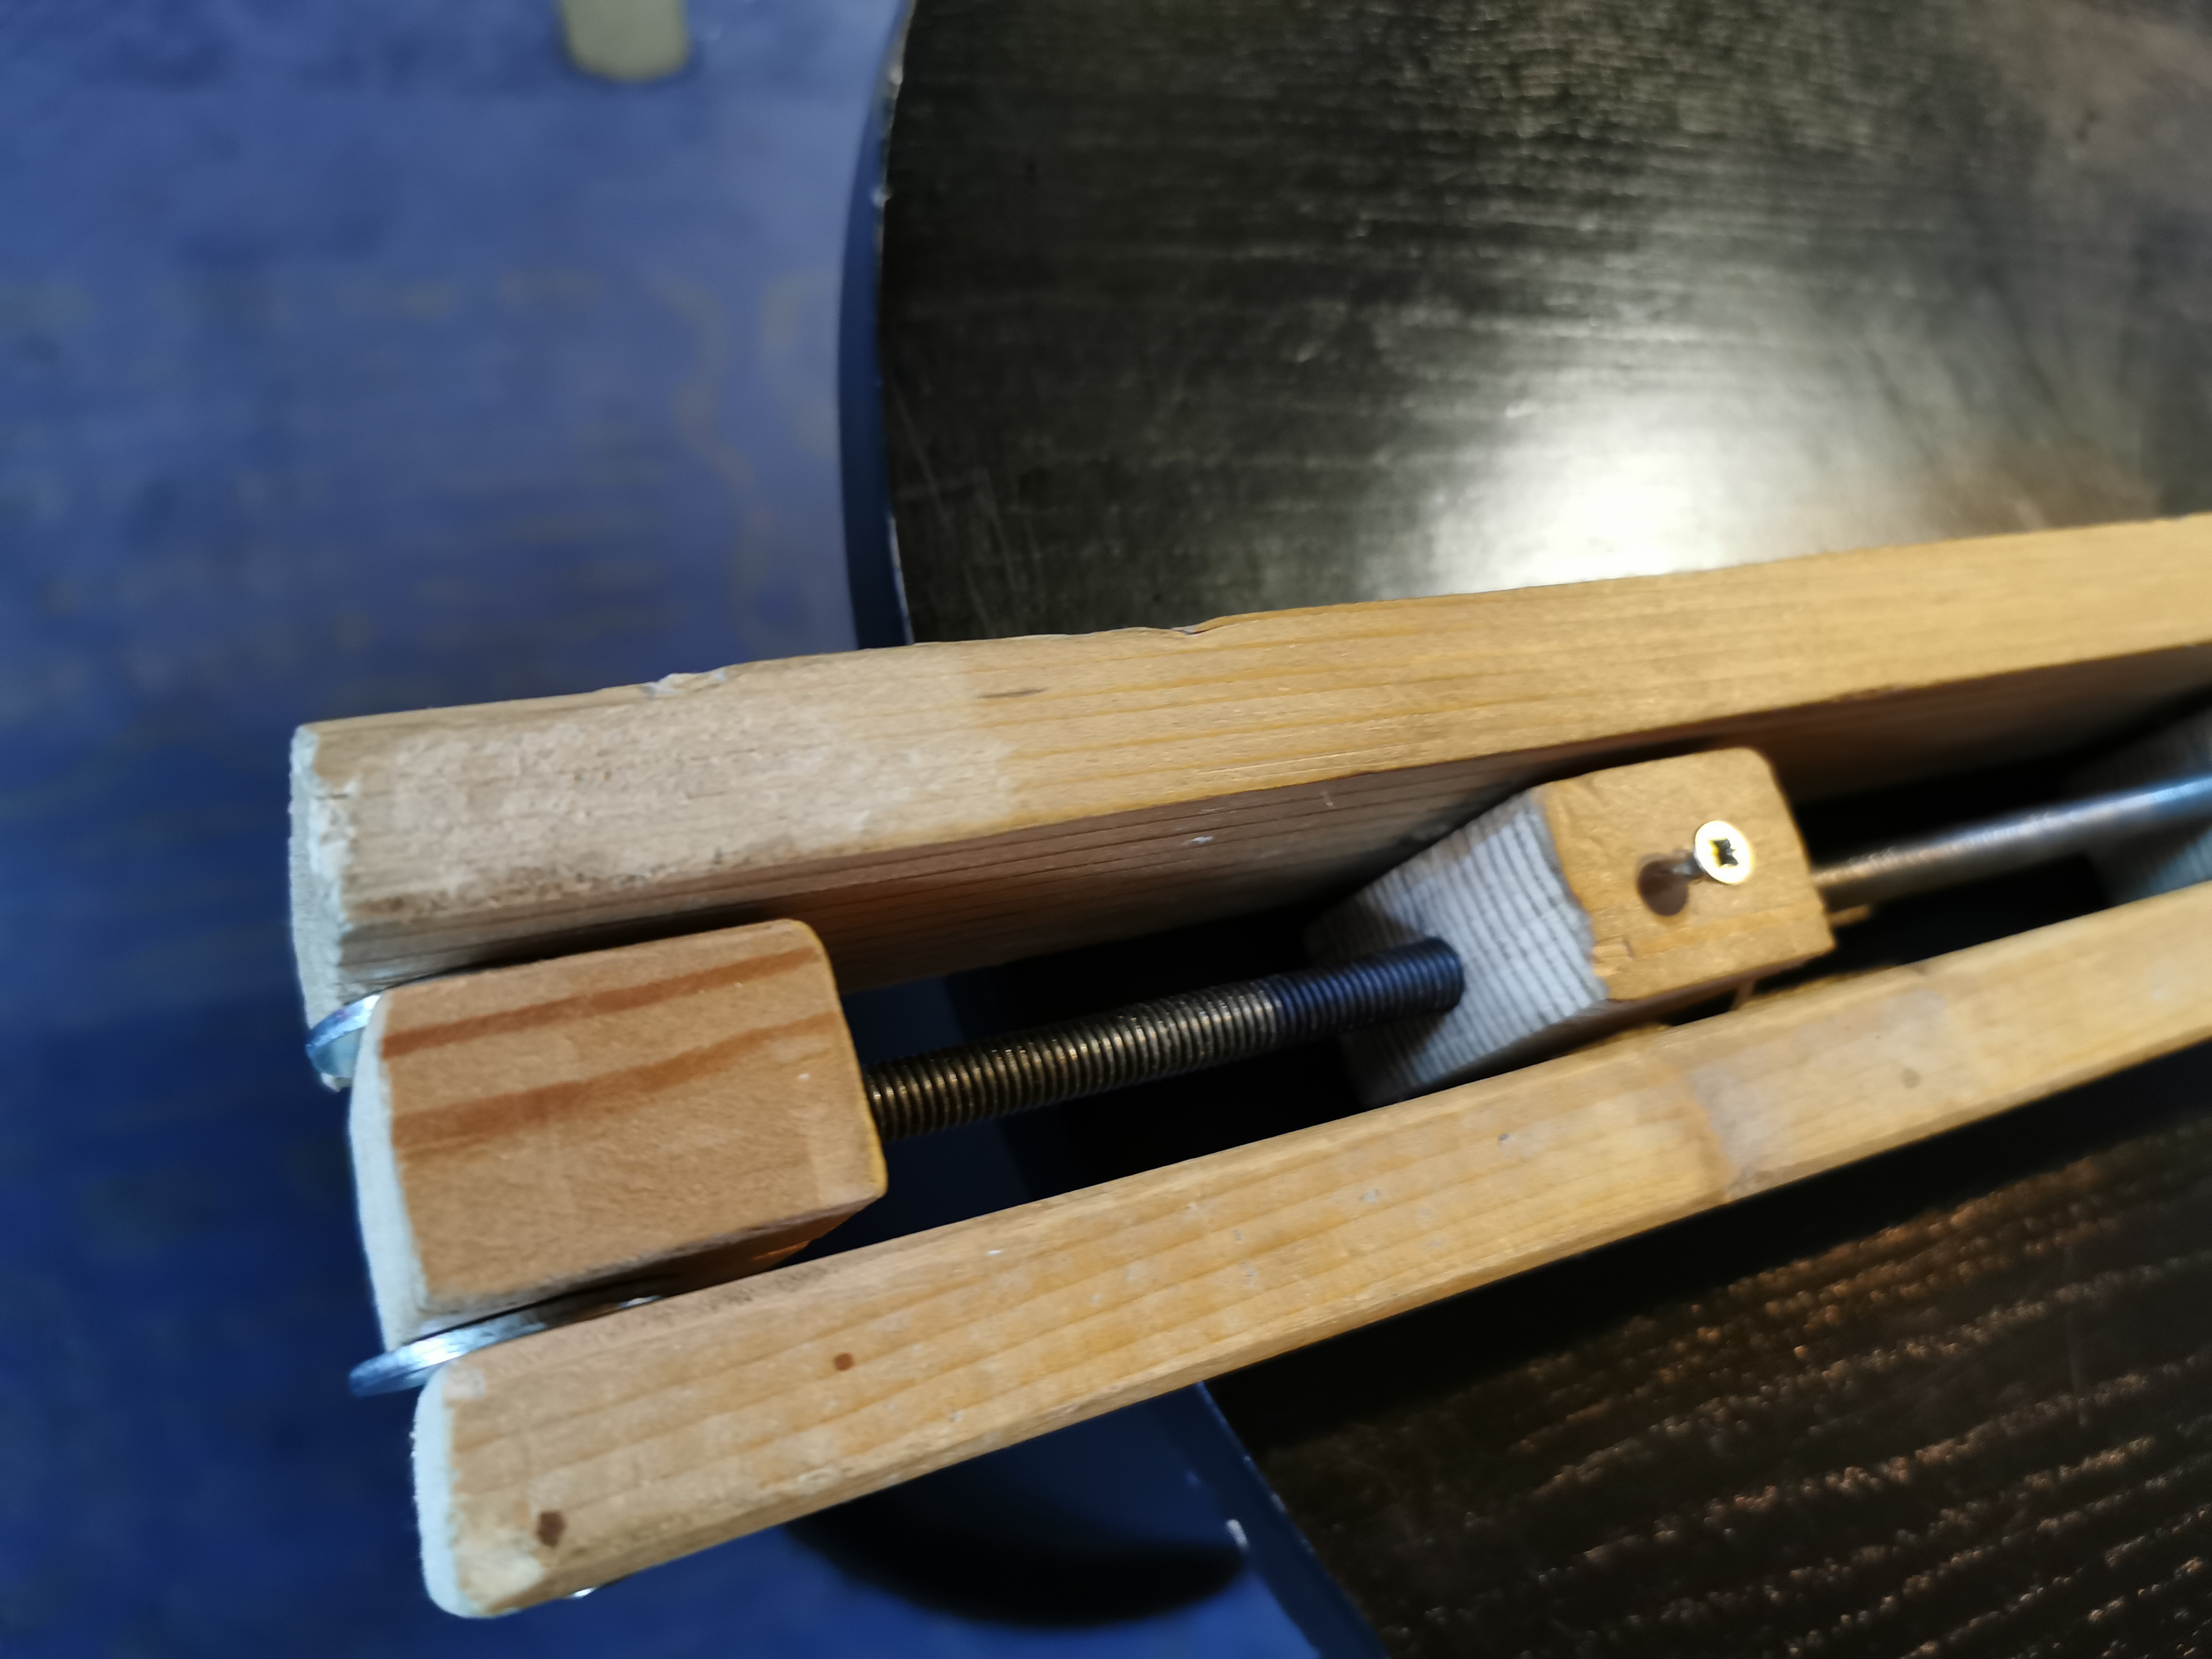
\includegraphics[width=\linewidth]{vegekozel.jpg}
\end{subfigure}%
~~
\begin{subfigure}[t]{.4\linewidth}
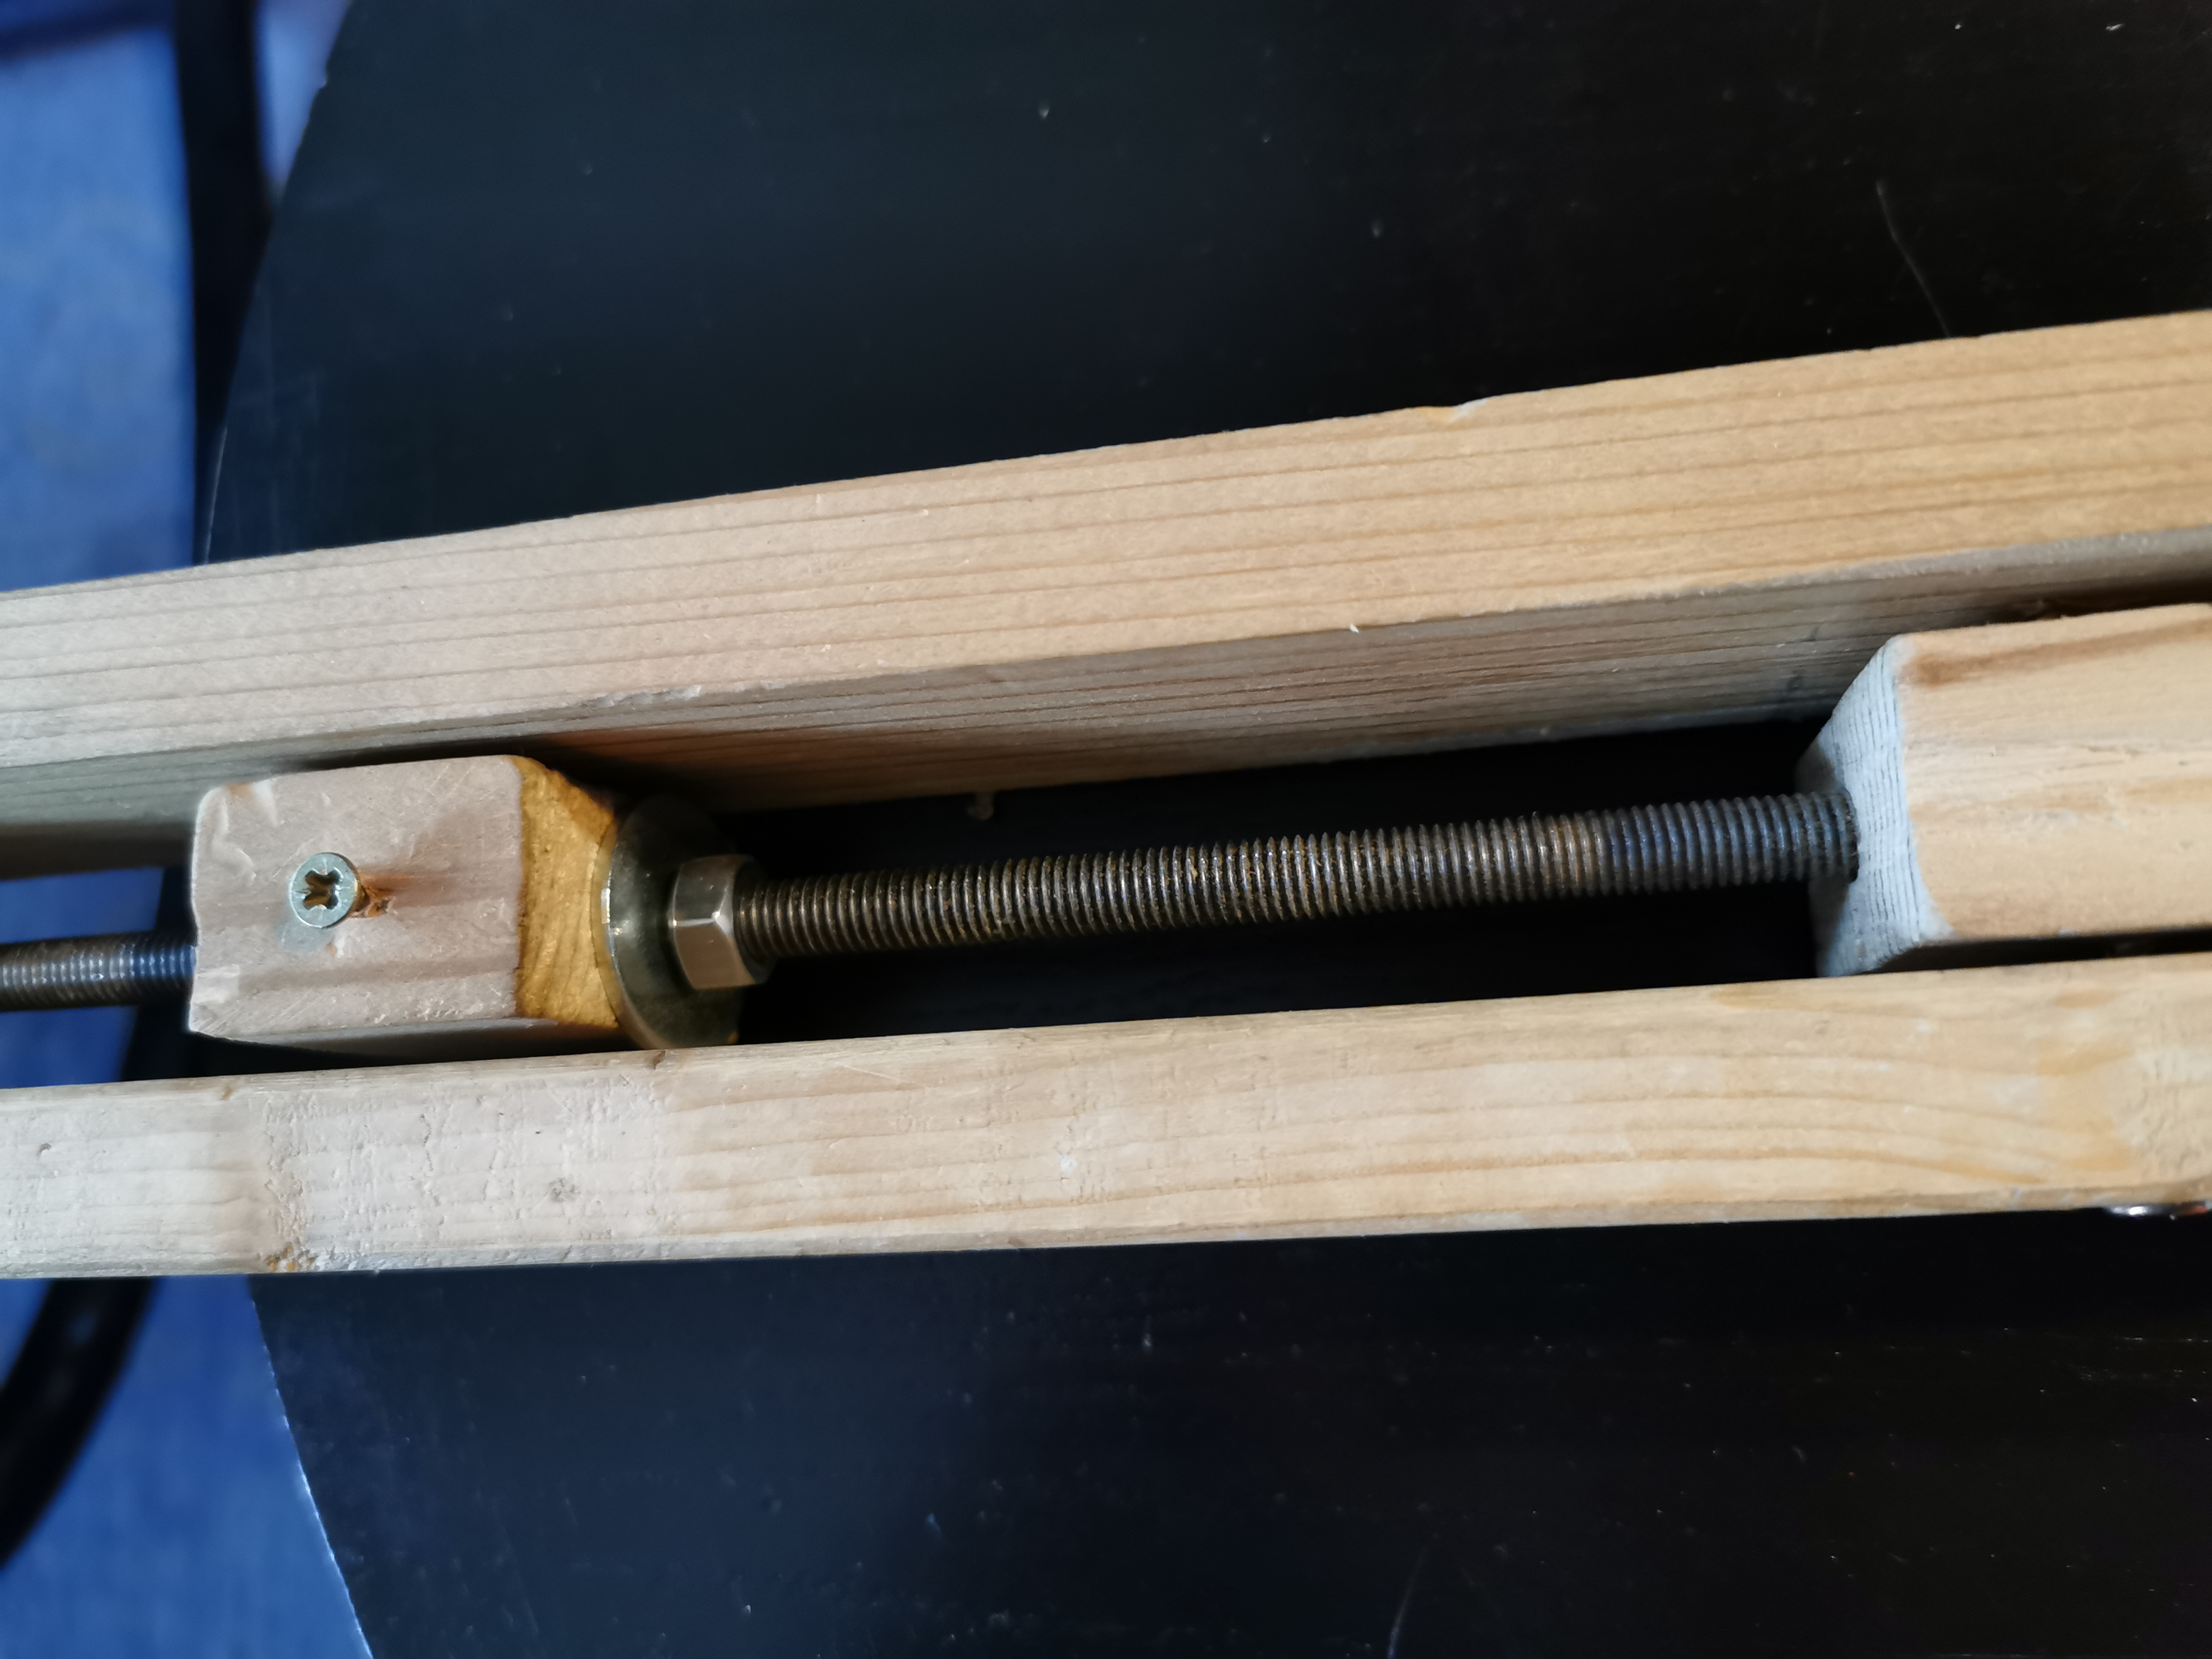
\includegraphics[width=\linewidth]{vegekozel2.jpg}
\end{subfigure}
\caption{}
\label{menetes}
\end{figure}

A méréshez egy A3 és egy E3 hárfahúrt használtuk. Azok hosszát a méréseinknél közepes, $30$\,N feszítőerőnél mértük meg, azokra $L_\text{A} = (72,5 \pm 0,5)$\,cm és $L_\text{E} = (80,5 \pm 0,5)$\,cm adódtak. Sűrűségnek az irodalmi értéket \cite{hur_surusegek}, $\rho = 1150$\,$\kgm$-t használtuk.

% ----------------------------------------------------------------
\subsection{Mérés menete}

A méréshez a két húr alapfrekvenciáit különböző feszítőerők mellett mértük, amit különböző súlyokkal értünk el. Figyeltünk arra, hogy a megfeszítésnél a feszítő kar vízszintes legyen, mert így pontos az erőkar áttétel A mérésnél a Fourier transzformációhoz \emph{Hanning} ablakot használtunk, viszont \emph{Ractangle} ablakkal is hasonló eredményeket kaphatunk. A mért alapfrekvenciákat és a feszítő erőket lejegyeztük.

A mérési eredményeket az \emph{Igor Pro} \cite{igor} szoftverrel értékeltük ki. Ugyanezt \emph{Excellel} \cite{excel} is meg lehet csinálni, viszont ott az illesztésnél nem lehet a mért adatoknak hibát megadni és az illesztésből kapott értékek hibájának kiszámolása is körülményes. Viszont ahhoz, hogy a mérés pontosságáról mondani tudjunk valamit, szükségünk van az eredmény hibájára is.

% ----------------------------------------------------------------
\subsection{Mérési eredmények}

A mérést két húrral is elvégeztük, a mért értékeket a \ref{hur_eredmenyek}.\ táblázatban láthatjuk.

\begin{table}[h!]
\centering
\begin{subtable}[t]{.5\linewidth}
\centering
\begin{tabular}{c | c}

$T$ (N) & $f_0$ (Hz) \\
\hline
 $9,8 \pm 0,5$ & $107,0 \pm 1,5$ \\
$19,6 \pm 1,0$ & $140,0 \pm 1,8$ \\
$29,4 \pm 1,5$ & $161,8 \pm 1,8$ \\
$39,2 \pm 2,0$ & $178,8 \pm 2,4$ \\
$49,0 \pm 2,5$ & $199,0 \pm 2,6$ \\
$58,8 \pm 2,9$ & $213,8 \pm 3,3$ \\
$68,6 \pm 3,4$ & $224,5 \pm 3,0$ \\

\end{tabular}
\caption{A3 húr}
\end{subtable}%
\begin{subtable}[t]{.5\linewidth}
\centering
\begin{tabular}{c | c}

$T$ (N) & $f_0$ (Hz) \\
\hline
 $9,8 \pm 0,5$ & $108,5 \pm 1,2$ \\
$19,6 \pm 1,0$ & $141,8 \pm 1,0$ \\
$29,4 \pm 1,5$ & $169,5 \pm 0,7$ \\
$39,2 \pm 2,0$ & $184,3 \pm 1,0$ \\
$49,0 \pm 2,5$ & $199,8 \pm 1,1$ \\
$58,8 \pm 2,9$ & $211,0 \pm 1,4$ \\

\end{tabular}
\caption{E3 húr}
\end{subtable}
\caption{}
\label{hur_eredmenyek}
\end{table}

Ezeket ábrázolva és a korábbiakban tárgyalt $f(T) = C \sqrt{T + T_0}$ alakú függvényt illesztve rájuk a \ref{f_vs_T}.\ ábrát kapjuk.

\begin{figure}[h!]
\centering
\begin{subfigure}[t]{0.5\linewidth}
\centering
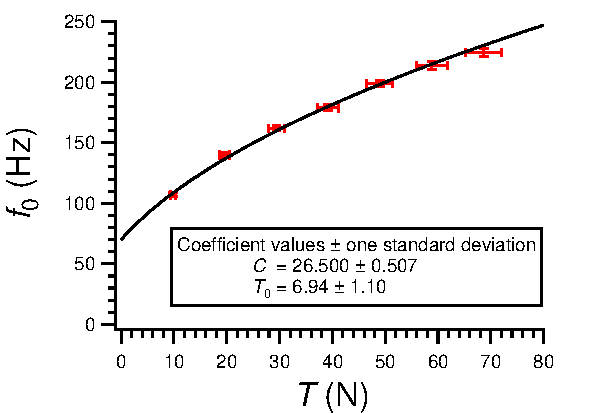
\includegraphics[width = \linewidth]{f_vs_T_A.pdf}
\caption{A3 húr}
\end{subfigure}%
\begin{subfigure}[t]{0.5\linewidth}
\centering
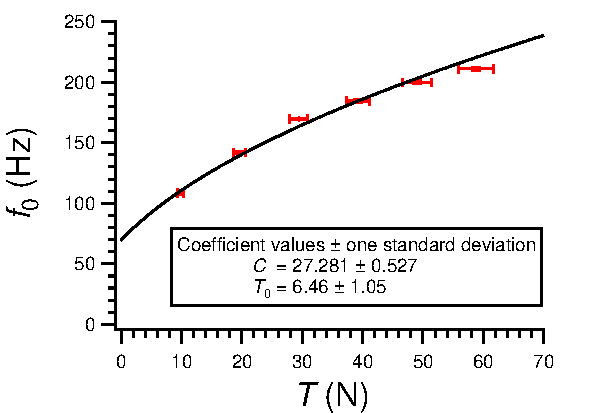
\includegraphics[width = \linewidth]{f_vs_T_E.pdf}
\caption{E3 húr}
\end{subfigure}
\caption{}
\label{f_vs_T}
\end{figure}

Az illesztésekből azt látjuk, hogy $T_0$ értéke mindkét esetben nagyjából ugyanakkora, ami megfelel a várakozásainknak. $C$ értékére pedig $C_\text{A} = (26,500 \pm 0,507)$ és $C_\text{E} = (27,281 \pm 0,527)$ adódnak. Ebből a
$$ d = \frac{1}{C L \sqrt{\rho \pi}} $$
képlet alapján számolhatjuk az átmérőt. A mért $L_\text{A}$ és $L_\text{E}$ értékeket is behelyettesítve $d_\text{A} = (0,866 \pm 0,018)$\,mm és $d_\text{E} = (0,758 \pm 0,015)$\,mm adódnak. Ezek hibájából azt mondhatjuk, hogy a mérés viszonylag pontos, a pontossága egy átlagos tolómérő pontosságához hasonló.

% --------------------------------
\subsubsection*{Méréskiértékelés Excellel}

Ha Excelt szeretnénk az adatok kiértékeléséhez használni, akkor az ábrázolásnál és illesztésnél másképp kell eljárnunk. Itt az A3 húrhoz tartozó mérési eredményeket fogjuk példaképpen kiértékelni.

Mivel az Excelben kevesebb opció van az illesztés paramétereinek megadására és azok rögzítésére, nem tudunk közvetlenül az $f_0$ - $T$ összefüggésre görbét illeszteni. Viszont ha az alapfrekvenciát négyzetre emeljük az
$$ f_0^2 = \frac{1}{d^2 L^2 \rho \pi} T $$
lineáris összefüggést kapjuk. Így az $f_0^2$ - $T$ összefüggést ábrázolva és arra egyenest illesztve megkaphatjuk az átmérőt. Az ábrázolást a \ref{excel_f2_vs_T}.\ ábrán láthatjuk.

\begin{figure}[h!]
\centering
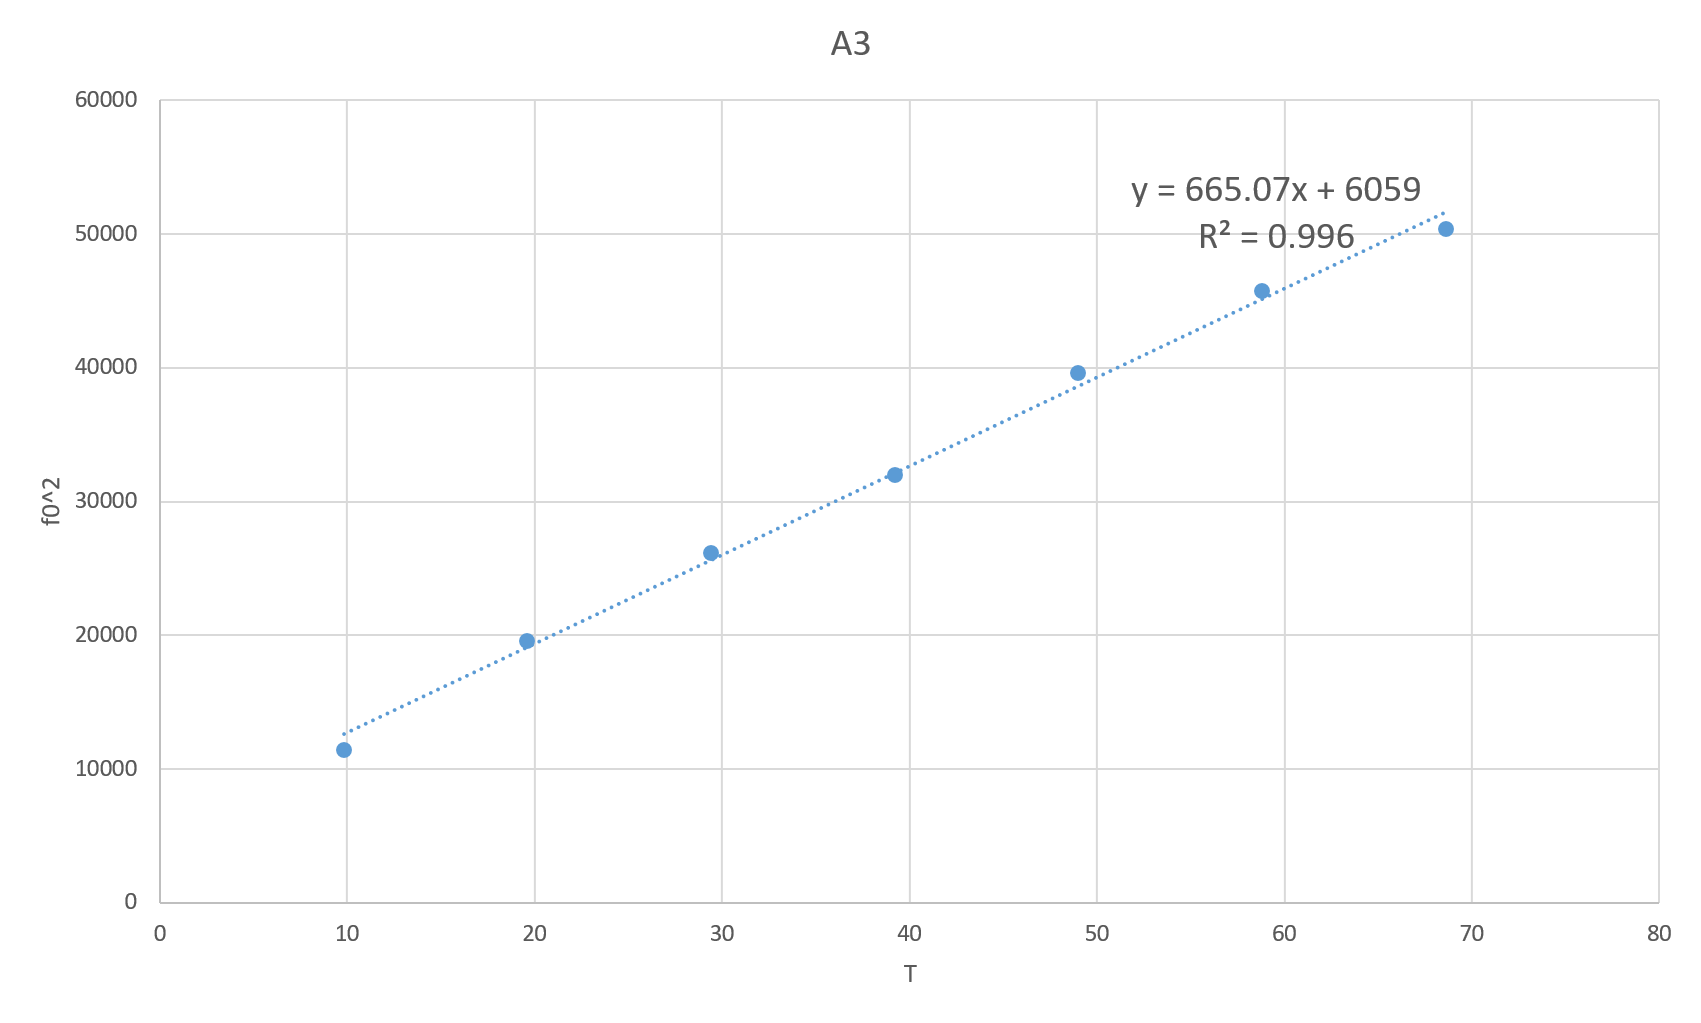
\includegraphics[width = 14cm]{excel_f2_vs_T.png}
\caption{}
\label{excel_f2_vs_T}
\end{figure}

Az illesztésből $C^2 = 665,07$ adódik, így $C = 25,789$. Ezzel az átmérőt kiszámolva $d = 0,890$\,mm adódik. Ez a korábban kiszámolt $d_\text{A}$ értéknek csak kétszeres hibakörnyezetébe esik bele, így azt mondhatjuk, hogy az így számolt érték csupán egy becslés.





% ================================================================
\newpage
\begin{thebibliography}{h!}

\bibitem{kisfiz1}
Vankó Péter: Kísérleti fizika 1.\ 10.6.\ fejezet \\
\href{http://physics.bme.hu/sites/physics.bme.hu/files/users/BMETE11AF42_kov/KisFiz1.pdf}
{\texttt{http://physics.bme.hu/sites/.../KisFiz1.pdf}}

\bibitem{mintamuszer}
Fizipédia: Állóhullámok megfeszített, rugalmas húrban \\
\href{https://fizipedia.bme.hu/index.php/\%C3\%81ll\%C3\%B3hull\%C3\%A1mok_megfesz\%C3\%ADtett,_rugalmas_h\%C3\%BArban}
{\texttt{https://fizipedia.bme.hu/index.php/ \\Állóhullámok\_megfeszített,\_rugalmas\_húrban}}

\bibitem{hur_surusegek}
\href{https://en.wikipedia.org/wiki/Nylon}
{\texttt{https://en.wikipedia.org/wiki/Nylon}}

\bibitem{igor}
\href{https://www.wavemetrics.com}
{\texttt{https://www.wavemetrics.com}}

\bibitem{excel}
\href{https://products.office.com/en-us/excel}
{\texttt{https://products.office.com/en-us/excel}}

\bibitem{github}
GitHub repository \\
\href{https://github.com/Il-Capitano/myDAQ-2019-2020}
{\texttt{https://github.com/Il-Capitano/myDAQ-2019-2020}}

\end{thebibliography}


\end{document}
